\documentclass[review]{elsarticle}

\usepackage{amsfonts,amsmath,amssymb,amsthm}

\usepackage{url}
%\usepackage{subfig}
\usepackage{multirow}
\usepackage{multicol}
\usepackage{floatrow}
\usepackage{paralist}
%\usepackage{lipsum}
\usepackage{graphicx}
\usepackage[center]{caption}
\usepackage{float}
\usepackage{csvsimple}
\usepackage{rotating}
%\usepackage{lscape}
\usepackage{pdflscape}
\usepackage{enumitem}
%\usepackage{cite}
% \usepackage{lstlisting}
\usepackage{listings}
\usepackage{url}
\usepackage{breakurl}
\usepackage[breaklinks]{hyperref}
% \usepackage[ruled,vlined]{algorithm2e}
%\usepackage{algorithmicx} 
% \usepackage{algorithmic}
\usepackage{algpseudocode}
\usepackage{algorithm}
%\usepackage{algcompatible}
\usepackage{xspace}

% \usepackage[center]{caption}
% \usepackage{rotating}
% \usepackage{subfig}
\usepackage{subfig,etoolbox}% http://ctan.org/pkg/{subfig,etoolbox}
\usepackage{lipsum}
\usepackage{titlesec}

\titlespacing\section{0pt}{12pt plus 4pt minus 2pt}{0pt plus 2pt minus 2pt}
\titlespacing\subsection{0pt}{12pt plus 4pt minus 2pt}{0pt plus 2pt minus 2pt}
\titlespacing\subsubsection{0pt}{12pt plus 4pt minus 2pt}{0pt plus 2pt minus 2pt}


\makeatletter
\AtBeginDocument{\patchcmd{\sf@subfloat}% <cmd>
  {\maincaptiontopfalse}% <search>
  {\maincaptiontoptrue}% <replace>
  {}{}}% <success><failure>
\makeatother
\usepackage[dvipsnames]{xcolor}

\makeatletter
\newcommand{\printfnsymbol}[1]{%
  \textsuperscript{\@fnsymbol{#1}}%
}

\makeatother

% Add a period to the end of an abbreviation unless there's one
% already, then \xspace.
\makeatletter
\DeclareRobustCommand\onedot{\futurelet\@let@token\@onedot}
\def\@onedot{\ifx\@let@token.\else.\null\fi\xspace}
%\usepackage{appendix}

%\usepackage[showframe]{geometry} %for two column image

\graphicspath{{./figures/}}
%\usepackage{pifont}
%\usepackage{graphicx,subfigure}
%\usepackage{IEEEtrantools}
%\usepackage{soul,color,
%\usepackage{tikz}
%\usepackage{authblk}
%\usepackage{textcomp}
%\usepackage{slashed}
%\usepackage{booktabs}
% \sethlcolor{yellow}
%\usepackage{amsopn}
%\usepackage{bbm}
%\usepackage{algorithm,algcompatible}
%\usepackage{algpseudocode}
%\usepackage{csvsimple,booktabs,siunitx}
%\usepackage{natbib}

%\usepackage[numbers]{natbib}


%\usepackage[inline]{enumitem}

\DeclareMathOperator*{\argmax}{\arg\!\max}% http://tex.stackexchange.com/q/83169/576z4
%\graphicspath{{img/}}
%\usepackage{euscript}
%\usepackage{eucal}
%\usepackage
%\usepackage{multirow}
%\usepackage[pdftex]{hyperref}
%\usepackage{lmodern}
%\hypersetup{pdfmenubar=true,colorlinks=no}
\newtheorem{theorem}{\bf Theorem}%[section]
\newtheorem{lemma}{\bf Lemma}
\newtheorem{claim}{Claim}
\newtheorem{proposition}{\bf Proposition}
\newtheorem{conjecture}{Conjecture}
\newtheorem{corollary}{\bf Corollary}
\newtheorem{definition}{\bf Definition}
\newtheorem{fact}{\bf Fact}
\newtheorem{example}{\bf Example}
\newtheorem{discussion}{Discussion}
\newtheorem{remark}{\bf Remark}
\newtheorem{algorithmm}{\bf Algorithm}
\newtheorem{assumption}{\bf Assumption}
\def\p{{\rm P}}
\newtheorem{experiment}{\bf Experiment}
\def\p{{\rm P}}
%\setlength{\topmargin}{-0.3in}
%\setlength{\textwidth}{6in} % can be up to 6.5
%\setlength{\textheight}{8.5in} 
%\setlength{\evensidemargin}{-.4in}
%\setlength{\oddsidemargin}{.3in}


\newcommand{\mc}[1]{\mathcal{#1}}
\newcommand{\mbb}[1]{\mathbb{#1}}
\newcommand{\bs}[1]{\boldsymbol{#1}}

\newcommand{\tr}{\text{tr}}
%\newcommand{\Pr}{\text{Pr}}

\newcommand{\vect}[1]{\boldsymbol{#1}}
\newcommand{\set}[1]{\mathcal{#1}}

\newcommand\tab[1][0.5cm]{\hspace*{#1}}
%--------------------------------------------------------------------
%--------------------------------------------------------------------
\newcommand{\ie}{{i.e.}\@\xspace}
\newcommand{\eg}{{e.g.}\@\xspace}
\newcommand{\etal}{{et al.}\@\xspace}
\newcommand{\Ie}{{I.e.}\@\space}
\newcommand{\Eg}{{E.g.}\@\xspace}


\newcommand{\MetaSwaption}{{meta swaption}\@\xspace}


%\renewcommand{\S}{Section~}
\newcommand{\Apn}[1]{{Appendix~#1}}

\newcommand{\fatemeC}[1]{{\color{red}Comment by Fateme:} {\color{blue}#1}}
\newcommand{\mojtabaC}[1]{{\color{red}Comment by Mojtaba:} {\color{blue}#1}}
\newcommand{\ahC}[1]{{\color{red}Comment by Amirhossein:} {\color{blue}#1}}
\newcommand{\melikaC}[1]{{\color{red}Comment by Melika:} {\color{blue}#1}}


% Keys are defined here:
\newcommand{\keyone} { \color{black}leader\@\xspace}
\newcommand{\Aone} {\color{black}contract funding\@\xspace}
\newcommand{\Atwo} { \color{black}master\@\xspace}
\newcommand{\Delegation} { \color{black}delegation\@\xspace}


\newcommand{\freeride} {{freeride}\@\xspace}

\newcommand{\nodeal} {{nodeal}\@\xspace}

\newcommand{\deal} {{deal}\@\xspace}

\newcommand{\discount} {{discount}\@\xspace}

\newcommand{\underwater} {{underwater}\@\xspace}

\newcommand{\scdg} {{strongly-connected directed graph}\@\xspace}
% \newcommand{\depsrc}{{ \color{VioletRed}{deposition-source} }}
\newcommand{\SwaptionOwner}{{owner}\@\xspace}



\newcommand{\genGraph} {\color{black} swaptions\@\xspace}
\newcommand{\keyoneOk} {{protected}\@\xspace}
\newcommand{\AtwoOk} {{integrated}\@\xspace}
\usepackage{lineno,hyperref}
\modulolinenumbers[5]

\journal{Journal of Blockchain: Research and Applications}

%%%%%%%%%%%%%%%%%%%%%%%
%% Elsevier bibliography styles
%%%%%%%%%%%%%%%%%%%%%%%
%% To change the style, put a % in front of the second line of the current style and
%% remove the % from the second line of the style you would like to use.
%%%%%%%%%%%%%%%%%%%%%%%

%% Numbered
%\bibliographystyle{model1-num-names}

%% Numbered without titles
%\bibliographystyle{model1a-num-names}

%% Harvard
%\bibliographystyle{model2-names.bst}\biboptions{authoryear}

%% Vancouver numbered
%\usepackage{numcompress}\bibliographystyle{model3-num-names}

%% Vancouver name/year
%\usepackage{numcompress}\bibliographystyle{model4-names}\biboptions{authoryear}

%% APA style
%\bibliographystyle{model5-names}\biboptions{authoryear}

%% AMA style
%\usepackage{numcompress}\bibliographystyle{model6-num-names}

%% `Elsevier LaTeX' style
\bibliographystyle{elsarticle-num}
%%%%%%%%%%%%%%%%%%%%%%%

\begin{document}

\begin{frontmatter}

\title{Capital-free Futures Arbitrage\tnoteref{mytitlenote}}
%\tnotetext[mytitlenote]{Fully documented templates are available in the elsarticle package on \href{http://www.ctan.org/tex-archive/macros/latex/contrib/elsarticle}{CTAN}.}

%% Group authors per affiliation:
%\author{Elsevier\fnref{myfootnote}}
%\address{Radarweg 29, Amsterdam}
%\fntext[myfootnote]{Since 1880.}

%% or include affiliations in footnotes:
\author[mysecondaryaddress]{Mojtaba Tefagh}
\ead{mtefagh@sharif.edu}

\author[mymainaddress]{Fatemeh Bagheri \corref{aaa}} 
\ead{fateme.bagheri95@student.sharif.edu}
% \thanks{\P \ Equal contribution}

\author[mymainaddress]{Amirhossein Khajehpour \corref{aaa}}
\ead{amirhosseinkh@ce.sharif.edu}

\author[mythirdaddress]{Melika Abdi \corref{aaa}}
\ead{melika.abdi@ee.sharif.edu}

\address[mysecondaryaddress]{ Department of Mathematical Sciences, Sharif University of Technology}
\address[mymainaddress]{ Department of Computer Engineering, Sharif University of Technology}
\address[mythirdaddress]{ Department of Electrical Engineering, Sharif University of Technology}
\cortext[aaa]{These authors contributed equally to this work}

\begin{abstract}
%\section{Abstract}
\label{sec:abstract}
Cryptocurrency futures contracts that can be traded and settled by cash are exposed to the centralized exchange single point of failure. On the other hand, derivatives and synthetic tokens under the custody of smart contracts have suffered extensively from security issues and economic vulnerabilities resulting from oracle price manipulations. The middleman, being a centralized exchange or a decentralized application, can be hacked or exploited as long as the user does not own the private keys to the underlying assets of the futures contract.

To the best of our knowledge, the only non-custodial solution proposed at the time of writing is atomic swaptions and their extensions. However, their efficiency is limited by the fact that the specified amount to be delivered by either party should be locked from the negotiation until the expiry date. We introduce a framework to overcome this limitation without compromising decentralization to enable capital-free atomic swaptions and prove several interesting properties of these financial instruments.
\end{abstract}

\begin{keyword}
decentralized finance \sep DeFi \sep HTLC\sep atomic swap \sep atomic swaption
\MSC[2010] 93A14
\end{keyword}

\end{frontmatter}


\linenumbers
\section{Introduction}
\section{Introduction}
\label{sec:w-motiv}

Many financial instruments have been established and implemented in traditional fiat-based markets; 
among them: options, futures, loans, bonds, derivatives, etc. In the past decade, the concept of cryptocurrency has opened a new gate toward the next generation of economy and finance. This field is still open to new ideas and introduces lots of implementation challenges for DeFi. 

By the invention of Ethereum smart contracts, so many decentralized financial applications were built which have resulted in the rapid growth of the ether market capital in general, and the total value locked in liquidity and lending protocols specifically \new{\cite{aave, maker, compound, wbtc, dydx}}. This demonstrates the urgent need for the blockchain counterpart of well-known financial instruments, especially loans, options, and \emph{decentralized exchanges} (DEX), and as a result, DeFi primitives are being demanded these days more than ever before \new{\cite{buterin2014next, uniswap, flashswaps, jelly}}. 

In the present study, we tackle this challenge and design primitives for decentralized futures market applications which in addition to Ethereum blockchain, work on first-generation blockchains like Bitcoin which do not support high-level Turing-complete scripting languages. Our bond issuance system and the corresponding procedures only require \emph{hash time locked contracts} (HTLC) as their building block and they do not rely on any oracle or third party interference. To the best of our knowledge \abcd is the first protocol in DeFi which offers an atomic unsecured cross-chain bond service.

As the pioneer in decentralization, the pseudonymous Satoshi Nakamoto has devised a new path towards the peer-to-peer payment systems which are counted as a disruptive innovation today \new{\cite{nakamoto2019bitcoin}}. Ethereum as the next generation of decentralized computing services enables writing smart contracts on an electronic ledger \new{\cite{buterin2014next}}. Later on, by the advent of ever-increasing blockchains, one may need to exchange assets across different networks. Through utilizing atomic swaps, two parties on different blockchains make an atomic contract which transfers asset between them \new{\cite{htlc-btctalk}}. Up until now, several previous works have extended the usage of atomic swaps in different ways. Herlihy designed a model for analyzing atomic cross-chain swaps and suggested a protocol that not only removes incentives for any set of parties to deviate from the protocol, but also guarantees that no conforming party ends with the underwater outcome and showed that HTLCs are enough to achieved this \new{\cite{herlihy2018atomic}}. Zamyatin \etal presented X{\footnotesize CLAIM} which is a swap frame work based on the atomic swaps that is faster and considerably cheaper than normal atomic swaps \new{\cite{8835387}}.
% Meyden \etal considered the term of atomic swap multi-party transactions using smart contracts in \cite{van2019specification}.
The idea of atomic cross-chain transactions in Ethereum sidechains was developed in \new{\cite{robinson2019atomic}}. The conflict caused by the concurrent execution of smart contracts was addressed to make an all-or-nothing atomic cross-chain commitment protocol in \new{\cite{zakhary2019atomic}}. Furthermore, Runchao \etal put a step forth by analyzing the fairness of atomic swaps and showed that the basic atomic swap is considerably more unfair compared to its equivalent contracts in the traditional market. Besides, they proposed two enhanced atomic swap protocols and justified their fairness \new{\cite{10.1145/3318041.3355460}}.
% (1) if all parties conform to the protocol, then all swaps take place, (2) if some coalition deviates from the protocol, then no conforming party ends up worse off, and (3) no coalition has an incentive to deviate from the protocol.
Liu proposed an atomic swaption component which works only using low-level scripting tools \new{\cite{liu2018atomic}}. Additionally, by utilizing his swaption component, offering fully decentralized futures contracts is no longer impossible \new{\cite{liu2018atomic}}.
Zie~\etal extended the atomic cross-chain swap contracts to a new method that does not need HTLCs and everything is managed by different party's signatures \new{\cite{zie2019extending}}.
% Furthermore, we propose two fair Atomic Swap protocols, one is for currency exchange and the other is for American Call Options. The quantification results show that the the Atomic Swap is much more unfair on cryptocurrencies than on stocks and fiat currencies in the same setting. 


% Most of mentioned systems have one thing in common: they are implemented for a turing complete bock chain and with the aid of smart contracts.
% In order to show the economical willingness towards the subject, some financial application implementations are mentioned below:

% Some developed solutions for applying these traditional economical applications to the world of crypto-currencies are:

% Some of the reputed DeFi applications are Compound, Maker DAO

% There are some developed solutions for applying these traditional economical applications to the world of crypto-currency.Here are some examples from


% \begin{itemize}
%     \item \textbf{ACO}: A protocol for decentralized and non-custodial trading of options \cite{aco}.
%     \item \textbf{Jelly Swap}: A peer to peer trading tool across different blockchains using atomic swaps \cite{jelly}.
%     \item \textbf{Uniswap}: A fully decentralized on-chain protocol for token exchanges on Ethereum that uses liquidity pools instead of order books \cite{uniswap}.
%     \item \textbf{Aave}: An open source and non-custodial protocol to earn interest on depositing and borrowing assets \cite{aave}.
%     \item \textbf{MakerDAO}: A decentralized credit platform on Ethereum that supports Dai, a stablecoin whose value is pegged to USD and backed in ETH or BAT \cite{maker}. 
%     \item \textbf{Compound}: An open-source money market protocol on Ethereum that lets users lend or borrow assets against collateral \cite{compound}. 
%     \item \textbf{Atomic Loan}: A lending platform that accepts trustless BTC collateral via custom Bitcoin scripts \cite{atomicLoan}. 
%     \item \textbf{DAI}: A decentralized stablecoin soft-pegged to the US Dollar \cite{maker}. 
%     \item \textbf{WBTC}: An ERC20 token that is backed 1:1 by bitcoin and opened the gate of trading bitcoin under ethereum blockchain \cite{wbtc}.
%     \item \textbf{dYdX}: An non-custodial trading platform on Ethereum geared toward experienced traders \cite{dydx}. 
    
% \end{itemize}

% For showing the growing investment interest in financial derivatives of crypto currencies, we can consider Fig.~\ref{fig:TVL-ACO} and \ref{fig:TVL-Uniswap} which are the overview of the money (in USD) locked in Uniswap and ACO and their fluctuations during the recent three months:
% \begin{figure}
%     \centering
%     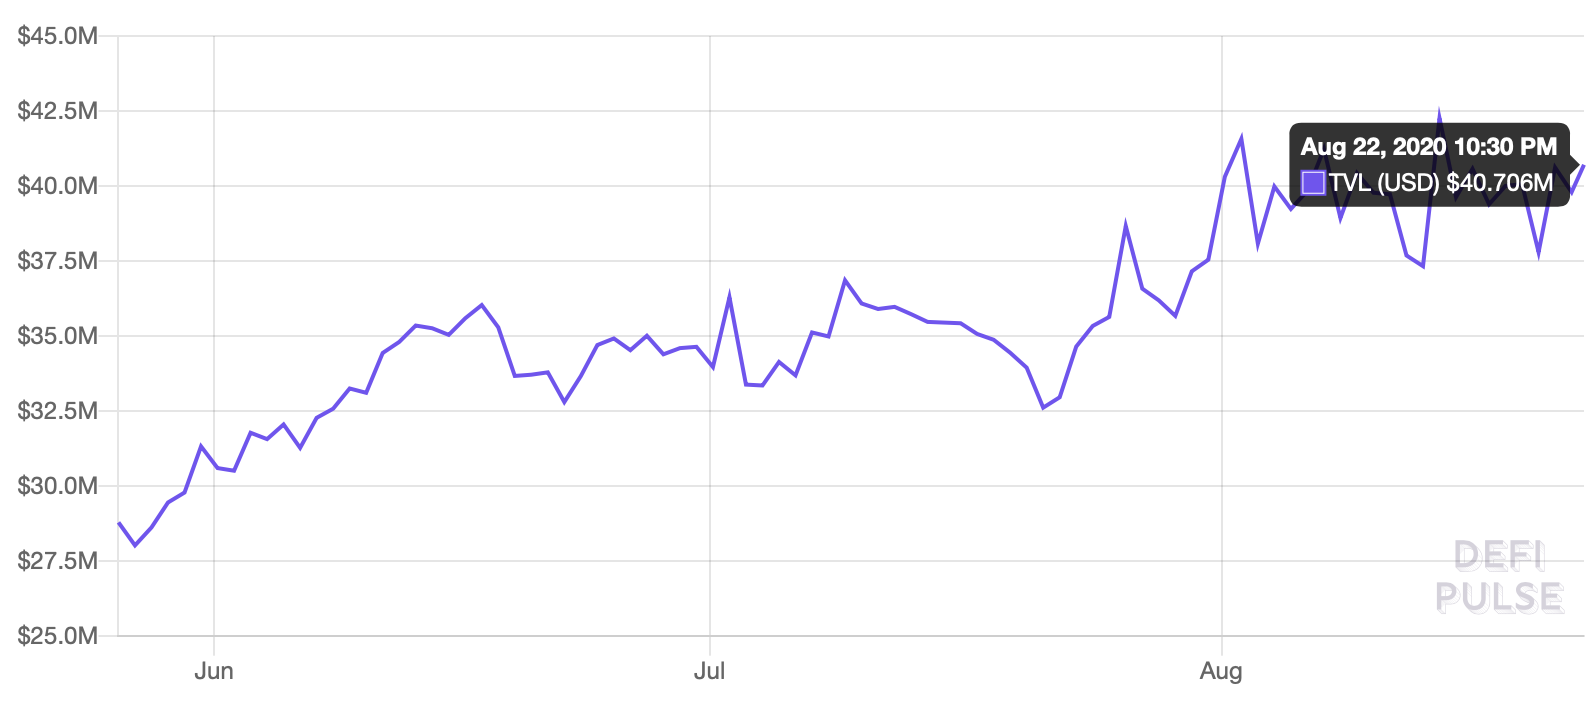
\includegraphics[width=\textwidth]{figures/dydx.png}
%     \caption{Total value locked (USD) in dydx \cite{dydx-cap}. Currently more than 40 M\$}
%     \label{fig:TVL-ACO}
% \end{figure}
% \begin{figure}
%     \centering
%     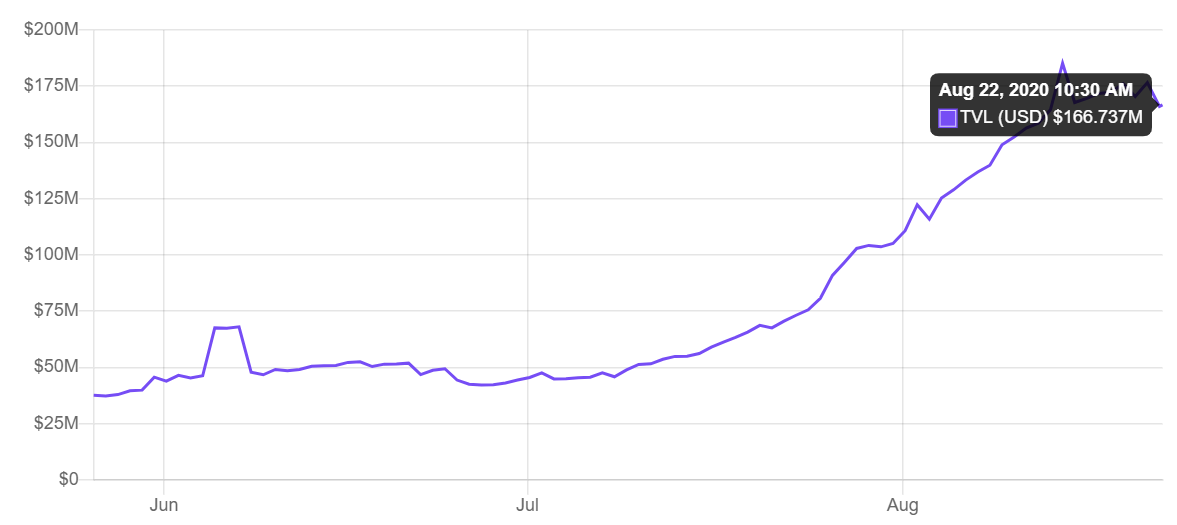
\includegraphics[width=\textwidth]{figures/TVL(USD)-uniswap-90.png}
%     \caption{total value locked (USD) in Uniswap \cite{uniswap-cap}. Currently more than 166 M\$}
%     \label{fig:TVL-Uniswap}
% \end{figure}





% \begin{tabular}{||c c c c c c||} 
%  \hline
%  BTC & ETH & DAI & AE & WBTC & USDC \\ [0.5ex] 
%  \hline\hline
%  20709.97 & 19216.02 & 9598.86 & 10226.57 & 209.33 & 3756.75 \\ [1ex] 
%  \hline
% \end{tabular}


 
The rest of this paper is organized as follows. First of all, in section~\ref{sec:abd} after defining the required terminology and presenting the other preliminaries of our work, we introduce the first \newfateme{model} of atomic bonded debt \newfateme{and discuss about the crucial requirements of an atomic bond service.} Later in section~\ref{sec:abcd}, we redesign our model to build the first practical \emph{atomic bonded cross-chain debt} (ABCD) primitive, \newfateme{and finally by adding additional features to it, we improve its stability across different market behaviours.}


% by using it afterwards, we build the \new{\emph{atomic bonded cross-chain debt} primitive (ABCD)}. 
% first practical version of ABCD component. Finally in the section~\ref{sub:seq-bond} we modify the ABCD to be used in the scenario of cross chain usecase.
% In Section~\ref{sec:relatedWorks}, we review some of the most important and recent studies on traffic classification with details. In Section~\ref{sec:Background}, we present the essential background on machine learning used in proposed methods, including deep learning and decision tree. In Section~\ref{sec:dataset}, we discuss the process of dataset collection and its various aspects, \eg, the reason for using two different datasets. Section~\ref{sec:Methodology} presents our proposed iterative procedure and the details of employed classifiers. The results of our experiments on the gathered data are elaborated in Section~\ref{sec:results}. Finally, we conclude the paper in Section~\ref{sec:conc}, briefing what we have learned throughout this study and how to improve it further.


\section{Atomic Swaption Revisited}
\label{sec:swaption}
To the best of our knowledge, Liu proposed the only implementation of atomic swaption which does not require either blockchain to support smart contracts \cite{liu2018atomic}. Afterward, Tefagh~\etal~ designed atomic bonded cross-chain debt (ABCD) as the first practical cross-chain bond platform in the form of atomic swaptions \cite{tefagh2020atomic}. In this paper, we have designed a more general model of atomic swaption named \emph{\MetaSwaption} which is abstractly shown in Fig~\ref{fig:moc-swaption}.

In what follows, we are going to briefly explain every module of the \MetaSwaption, and through the rest of this paper, we will use this general form as the building block for making some new application-specific swaptions.

\begin{figure}
    \centering
    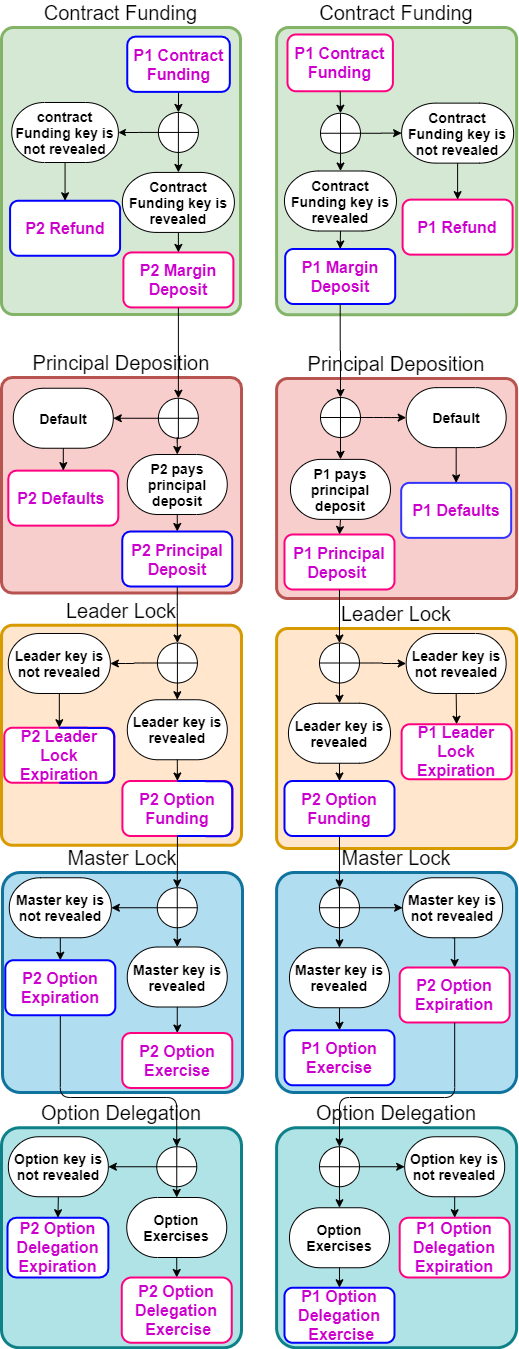
\includegraphics[width=\textwidth,height=\textheight,keepaspectratio]{figures/meta-swaption.png}
    \caption{General overview of the \MetaSwaption}
    \label{fig:moc-swaption}
\end{figure}

Similar to atomic swap and atomic swaption, HTLCs are used so that a party can make decisions by revealing a secret before a locktime or letting the locktime expire. In \MetaSwaption also there are four types of such secrets:
\begin{itemize}
    \item \Aone key
    \item \keyone key
    \item \Atwo key
    \item \Delegation key
\end{itemize}

Note that in HTLC contracts, generaly the locktime of the holder of the secret has to be greater than the other party.
%\ahC{It has to be greater}
% We call the one who buys the swaption, the swpation \SwaptionOwner. In our cases it is mostly Alice.

In the Fig~\ref{fig:moc-swaption}, a \MetaSwaption is 
divided into five different parts, each representing a particular stage in the swaption process. 

Note that in every module introduced in this paper, all transactions in the execution process are exchanged and signed by their corresponding parties before anything goes on chain. During this not-yet-confirmed transactions sharing, all parties are assured that no one can steal their money.


\begin{itemize}

    \item \textbf{Contract funding}: The funding for the swaption buyer (swaption owner) consists of premium and for the seller only margin. Depending on application, the \SwaptionOwner may include margin in her funding.
    The \SwaptionOwner has a relatively small amount of time to reveal \Aone key to buy the option. If she buys the option, premium goes to the seller and margins go to the principal deposition contracts.
    %  Each party sends his margin to a HTLC contract. The swaption buyer also pays a premium to buy the option from the seller. After the exchange of funding transactions, it is time for the swaption buyer to decide weather she buys the option or not. If she reveals the \Aone key, premium goes to the seller and margins go to the margin deposit contracts.
    
    \item \textbf{Principal deposition}: After buying the swpation, each party has to deposit his principal within a specified time interval. If both parties cooperate, the next stage begins.
    The principal deposition transactions might have sighash type of any-one-can-pay\footnote{ANYONECANPAY} since nobody knows all of its inputs in the first place. In this case, since we do not know all the inputs of this transaction at the time of signing, we would not have the correct transaction ID \cite{bip143}. Therefore, we can not create the transactions that get their inputs form this transaction until we discover what all the inputs of the this transaction are going to be. These inputs are only known at the time of broadcasting, not at the time of creating the transactions. So, at the time of creating the transactions in the next stage, the ID of the principal deposition transaction is unknown.
    
    \item \textbf{Leader lock}: Depending on the application, the swaption \SwaptionOwner may decide to use a portion of her option duration as the allowed period of her late principal deposition in order to make money for her principal. In this stage, the party who deposits his principal earlier, \keyone key holder, locks his principal. After assurance of the owner's principal deposition, he is expected to reveal \keyone key determining if the swaption goes to the next stage or not.
    As mentioned in the last stage, the ID of the input of the transactions of this stage is not known at the time of creating. Thus, we have to use the sighash type of no-input\footnote{NOINPUT}\cite{bip118} that allows us to create a transaction where none of its inputs are known. So, by this sighash we can create the transactions in the leader lock stage without any inputs. Later, at the time of broadcast, since the inputs of the principal deposition transaction are known and consequently we have its ID, we can use this transaction as an input for the transactions of the leader lock stage and broadcast them.
    
    \item \textbf{Master lock}: In this stage, the \SwaptionOwner (\Atwo key holder) chooses weather she exercises the option or not using \Atwo key. By exercising the option, principals are exchanged and the swaption ends. By not revealing \Atwo key, letting the locktime expire, next stage begins. Like the last stage, since the inputs of the parent transaction of the transactions of this stage are not clear, we have to use the no-input sighash.
    
    \item \textbf{Option delegation}: This stage might be utilized in certain use-cases such as futures arbitrage discussed later. For fixing the problem of cyclic locktimes in master lock stage, we develop a method to delegate the option from \SwaptionOwner to another desired party. The newly promoted party can later decide the execution of the swaption by the \Delegation key. In this stage, like last two stages we have to use the no-input sighash.

    % \item \textbf{Trust box}: In some cases, i.e. futures arbitrage, the \SwaptionOwner needs to transfer the right of signing some transactions to a party other than swaption buyer or seller. The extents of trust box may differ for each use-cases of \MetaSwaption instances.
    % \ahC{Is this paragraph needed anymore?}
\end{itemize}

When using the no-input sighash, the party signs the transaction without specifying its inputs, so a malicious party has the ability to give any UTXO that belongs to the public key of this party. Hence, each party has to create a separate public key for each transaction that she makes.
Using the stages described above, we can generate new instances of \MetaSwaption targeting swaptions or bonds. Based on different goals, we can choose which of these stages appear in our instance. In the following subsections, we describe different swaptions devised for a variety of use-cases:
\begin{itemize}
    \item Early deposition swaption
    \item Late deposition swaption
    \item Margin-free limited swaption
\end{itemize}
Notice that in Fig~\ref{fig:swaption-early-deposition}, Fig~\ref{fig:swaption-late-deposition}, and Fig~\ref{fig:swaption-margin-free-limited} the locktimes $P$,$T$,$M$,$E$, and $T'$ are calculated with respect to  a common origin of time. In other words, the current time of the swaption establishment has to be added to all the locktimes shown in these stages, because they are not relative but absolute times. 
% Each of these components has different procedure. For further analysing the effectiveness of each component, we design a time elapsed experiment aiming to analyse the worst case running time of them.


% \begin{experiment}
% {Time Elapsed}\\
% Given $p_{buyer}$ and $p_{seller}$ the buyer and the seller of the component $\mathcal{C}$, the $\mathcal{T}[\mathcal{C}]$ is the minimum spend locktime during the execution runtime of $\mathcal{C}$ if $p_{seller}$ adversarially waits in every steps until the last moments.
% \end{experiment}

% We discus the second type in detail. The other types are discussed in \Apn{\ref{app:conv-swaption}} and \Apn{\ref{app:margin-free-swaption}}.

% \ahC{Somewhere we have to mention that we split the option time into two parts, one is time for revealing \keyone key and the other one is \Atwo key. Then we can say that Alice is settling other swaptions in the case of arbitrage during option time.}



\subsection{Early Deposition Swaption}
\label{app:conv-swaption}

This type of swaption is the conventional form that is first introduced in \cite{liu2018atomic}. Alice wants to exchange her ACoins with Bob's BCoins. We rebuild this type with our \MetaSwaption extended form in the way depicted in Fig~\ref{fig:swaption-early-deposition}. We begin analysing each stage of this type by explaining every possible scenarios as follows:

\begin{itemize}
    \item \textbf{Contract funding}: Alice and Bob broadcast their funding transactions. Alice's includes margin and premium and Bob's includes margin worth equal to Alice's margin.
    
    \item \textbf{Principal deposition}: In this stage, Bob is waiting for Alice to deposit her principal. There are two possible scenarios:
    \begin{itemize}
        \item Alice does not deposit her principal. In this case, Bob also defaults and their margins are exchanged.
        \item Alice deposits her principal but Bob does not. In this case, Alice is in master lock stage. So, she reveals \Atwo and takes Bob's margin besides her own principal.
        % Alice is already in option contract stage and she can take the ownership of both her principal and Bob's margin by revealing the \Atwo key and broadcasting Bob's default transaction.
    \end{itemize}
     But if Bob fails to deposit his principal, 
    
    \item \textbf{Master lock}: If both parties go to this stage, Alice can then use her option as mentioned earlier.
\end{itemize}

\begin{figure}
    \centering
    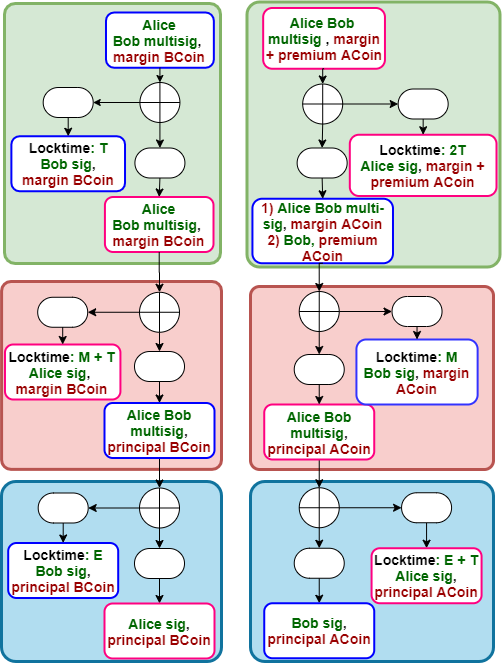
\includegraphics[width=\textwidth]{figures/early dep.png}
    \caption{Early deposition swaption where the buyer (Alice) deposits her principal earlier than the seller (Bob). The pink-bordered transactions are broadcasted by Alice and the blue-bordered ones by Bob.}
    \label{fig:swaption-early-deposition}
\end{figure}
% \ahC{Shall we mention that 546 Satoshis can not be counted as margin?}


\subsection{Late Deposition Swaption}
In this type of swaption the swaption \SwaptionOwner, Alice, needs the seller, Bob, to deposit his principal before her, so that she can settle other deals on other contracts before depositing her principal in this swaption. Alice can exploit this type of swaption in the situations where she does not own enough budget for her principal and she is going to make the required amount of capital using what she has takes from Bob. Since Bob has to wait a longer time for Alice to deposit, Alice has to pay more amount of premium compared to the early deposition swaption.
One example use-case can be the futures arbitrages which will be discussed later. The overview of this swaption is shown on Fig.~\ref{fig:swaption-late-deposition}.

\begin{itemize}
    \item \textbf{Contract funding:} The two parties broadcast their funding transactions. Alice includes margin in her funding and an amount of guarantee is added to Bob's funding besides his margin. We can use this guarantee amount to punish Bob in case of cheating. If he behaves normally, the guarantee will return back to him. The amount of guarantee is negotiable depending on the use-case.
    
    \item \textbf{Principal deposition:} When this stage begins Alice is waiting for Bob to deposit his principal. If Bob defaults, then Alice has two options to punish him:
    \begin{itemize}
        \item She defaults, loses her margin and takes Bob's guarantee and margin.
        \item She deposits her principal and enters the next stage.
    \end{itemize}

    \item \textbf{Leader lock}: 
    There are four possible scenarios:
    \begin{itemize}
        \item In the last stage, Bob deposited his principal but Alice did not. Now Bob does not reveal \keyone key, so that Alice's margin is exchanged with Bob's margin.
        \item Both have deposited their principals and Bob does not reveal \keyone key. Broadcasting the Alice's leader lock transactions, Alice gets Bob's guarantee.
        \item In the last stage, Alice deposited her principal but Bob did not (Second way to punish Bob). Now Alice broadcasts the Alice's leader lock expiration transaction and takes all of her principal back in addition to Bob's margin and guarantee that she has previously taken in the last stage. 
        \item Both have deposited their principals. Bob reveals \keyone key and take back his guarantee. Afterward, they go to the next stage.
    \end{itemize}
    
    \item \textbf{Master lock}: It is the time for Alice to use her option. She either exercises and principals are exchanged or reveals nothing and each party gets his principal back.
\end{itemize}


\begin{figure}
    \centering
    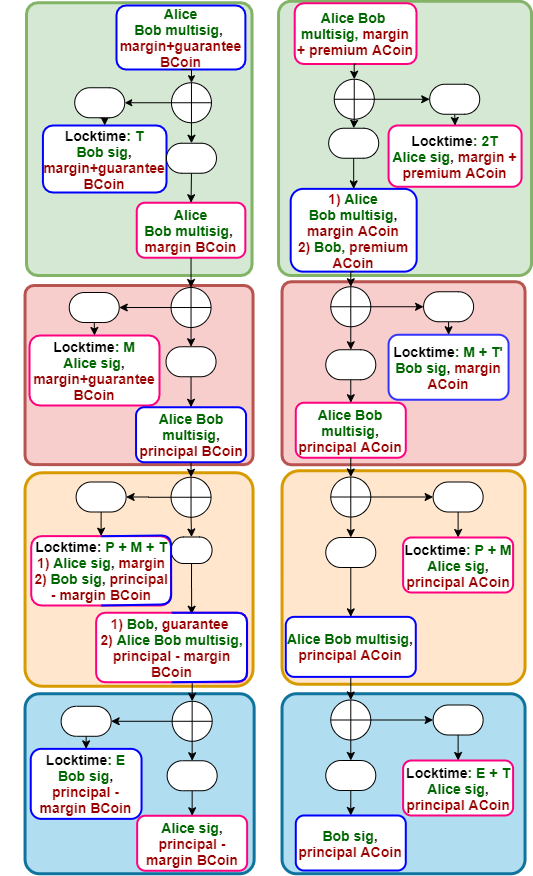
\includegraphics[width=\textwidth,height=0.93\textheight,keepaspectratio]{figures/late dep.png}
    \caption{Late deposition swaption where the seller (Bob) deposits his principal earlier than the buyer (Alice). Pink-bordered transactions are broadcast by Alice and blue-bordered ones by Bob.}
    \label{fig:swaption-late-deposition}
\end{figure}

% Note that since Bob's only incentive is the premium (and not the margin), it is not possible that Alice uses this swaption alongside with other swaptions. For instance, in the case that Alice uses Bob's principal as her principal in another swaption, Bob can cheat on Alice by pretending to be a different person and act as the other party in the second swaption as well as the first one. Then he can steal Alice's premium in the second swaption by not exposing the \keyone key. 
% Later we will prove that Alice can only use one premium guarantee in a set of swaptions which are expected to be exercised in one run simultaneously. Because every run must have only one \keyone and \Atwo and \Aone key which is impossible when we use multiple premium guarantee boxes.
% It is not possible to allow Alice to send the premium of other swaption in directly with usage of another Premium Guarantee 
%\ahC{This section is changed and it is no longer standalone. Still move to appendix?}
% The detailed process of this swaption is written in \Apn{\ref{app:margin-free-swaption}} 
% \ref{app:margin-free-swaption}.



% \subsection{Atomic Non-collateralized Loan}
% A modification of the {\it Late-Deposition swaption} in which Alice does not have to deposit any margin before she gets Bob's principal has the functionality of a loan with no collateral needed. As mentioned in \cite{liu2018atomic} it is not possible to have no margin for the buyer if the parties are on different blockchains. \fatemeC{explain more} Hence, in order to have this loan, the parties have to be on the same chain. 



\subsection{Margin-Free Limited Swaption}

\label{app:margin-free-swaption}
Until now, it was believed that Alice's margin deposit is necessary due to the limitations of HTLCs \cite{liu2018atomic}. In this work, we propose a novel approach which allows Alice to participate in a swaption without depositing any margin.
In the beginning of contract, Bob deposits an amount of BCoin as guarantee which is sent to Alice directly by revealing \Aone key. Alice also adds an amount of ACoin equal to Bob's guarantee to her premium, though none of them will be directly sent to Bob. Later, the premium and guarantee go to Bob in all possible situations except where Bob refuses to reveal the \keyone key when Alice does not default, then he will be punished by not getting back his guarantee.
% In Fig~ \ref{fig:swaption-margin-free-limited} we use our getting a guarantee money from Bob to build the {\it Margin Free} swaption.
% In this type besides premium, Alice deposits an amount of ACoiun equal to Bob's guarantee. Her premium is not paid directly after revealing of \Aone key, but instead will be locked until Bob acts honestly up to end of the Leader Lock stage.
% Later the premium goes to Bob in all possible situations except where Bob refuses to reveal the \keyone key and he will be punished by not paying back his guarantee. 
The amount of guarantee can vary depending on the Alice's need. In next section, we will explain the limitation imposed on the amount of guarantee in details. The execution procedure of the margin-free swaption is as follows:
\begin{itemize}
    \item \textbf{Contract funding}: Bob pays his margin plus an amount of guarantee which prevents him from cheating in later stages. Alice also pays extra premium which in the case of Bob's honest behaviour pays back the guarantee to Bob. Guarantee in the Bob's section is directly sent to Alice after revealing the \Aone key. 
    
    \item \textbf{Principal deposition}: This stage is the same as previous principal deposition stages for Bob. He has M locktime to deposit his principal. If he does not, Alice takes his margin. In Alice's section, either she defaults and gives Bob the premium or she deposits her principal and goes to the next stage waiting for Bob to reveal the \keyone key.
    % \item \textbf{Premium Guarantee}: Either Alice defaults and gives Bob the premium or she deposits her principal and goes to the next stage waiting for Bob to reveal the \keyone key.
    
    \item \textbf{Leader key}: If Bob has not deposited his principal until M locktime, Alice will also avoid depositing her principal and gives Bob the premium and ACoin guarantee while getting his margin from him.
    % and Alice has two options ahead: 1)She deposits her principal before M + T, then broadcasts the \keyone key expiration transaction, in which her premium is refunded. Therefore, if Bob defaults and Alice does not, there would be no premium for Bob. In any other situation he gets the premium. 
    If both parties have deposited their principals when this stage begins, Bob's decision whether to reveal the \keyone key or not, determines the future of the swaption. If he refuses to reveal, he takes his own money back and Alice takes her own money including premium back. In this case, Bob loses his guarantee as a punishment. Otherwise, if he reveals the \keyone key, they both go to the next stage waiting for Alice to exercise her option. Additionally, by revealing the \keyone key, Bob finishes his task and it is the time to send back his guarantee. Hence at the end of this stage, Bob's guarantee will be paid back to himself.
    
    \item \textbf{Option funding}: This stage is similar to the last versions of swpation.
\end{itemize}

\begin{figure}
    \centering
    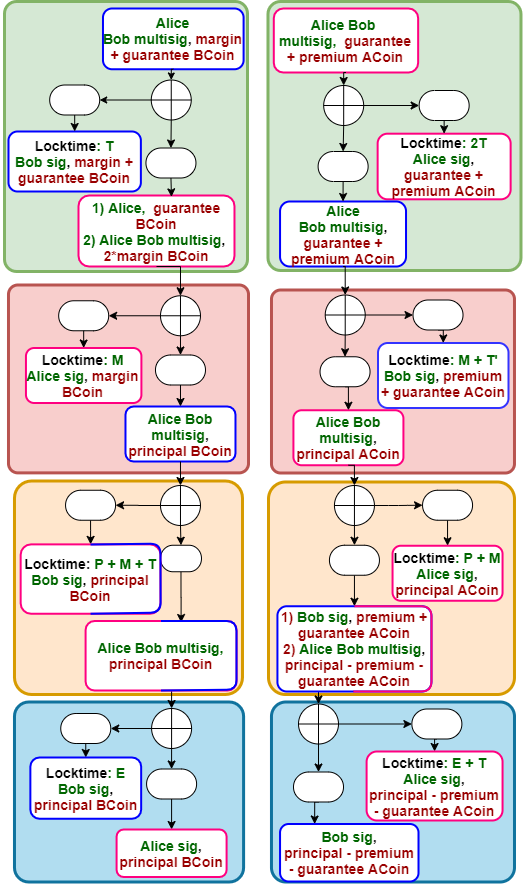
\includegraphics[width=\textwidth,height=0.93\textheight]{figures/swaption-margin-free.png}
    \caption{Margin-free limited swpation where the buyer (Alice) is not supposed to deposit any margin. Pink-bordered transactions are broadcasted by Alice and blue-bordered ones by Bob.}
    \label{fig:swaption-margin-free-limited}
\end{figure}
% \fatemeC{mention auction as an application for the margin-free swaption. you can use the aucion section primarily written}

Locktimes in all of these swaptions have to stick to some general rules: 
\begin{itemize}
    \item $T$ is the minimum amount of time or number of blocks needed for a mined transaction to be confirmed. In bitcoin it is $6$ blocks which is approximately achieved in 1 hour.
    
    \item $M$ is the time for Bob to deposit principal. Hence, can be equal or greater than $T$.
    
    \item $T'$ can be relatively large, since it gives Alice the time she needs to deposit her principal.
    
    \item $P$ is the locktime that Bob has to reveal the \keyone key. This has to be larger than $T'$ so that Alice has to deposit before Bob's revealing time elapses.
    
    \item $E$ is the time for Alice's option exercise which can be relatively large, since it is an option.
\end{itemize}
Note that we use $T$ to make two locktimes differ in a reasonable amount of time to prevent cheating. However, this is the minimum difference needed. Hence, everywhere $T$ is used, we can replace it with different larger values. We use $T$ for simplicity though.
\section{Futures Arbitrage}
\label{sec:arbitrage}
\begin{figure*}[!ht]
    \centering
    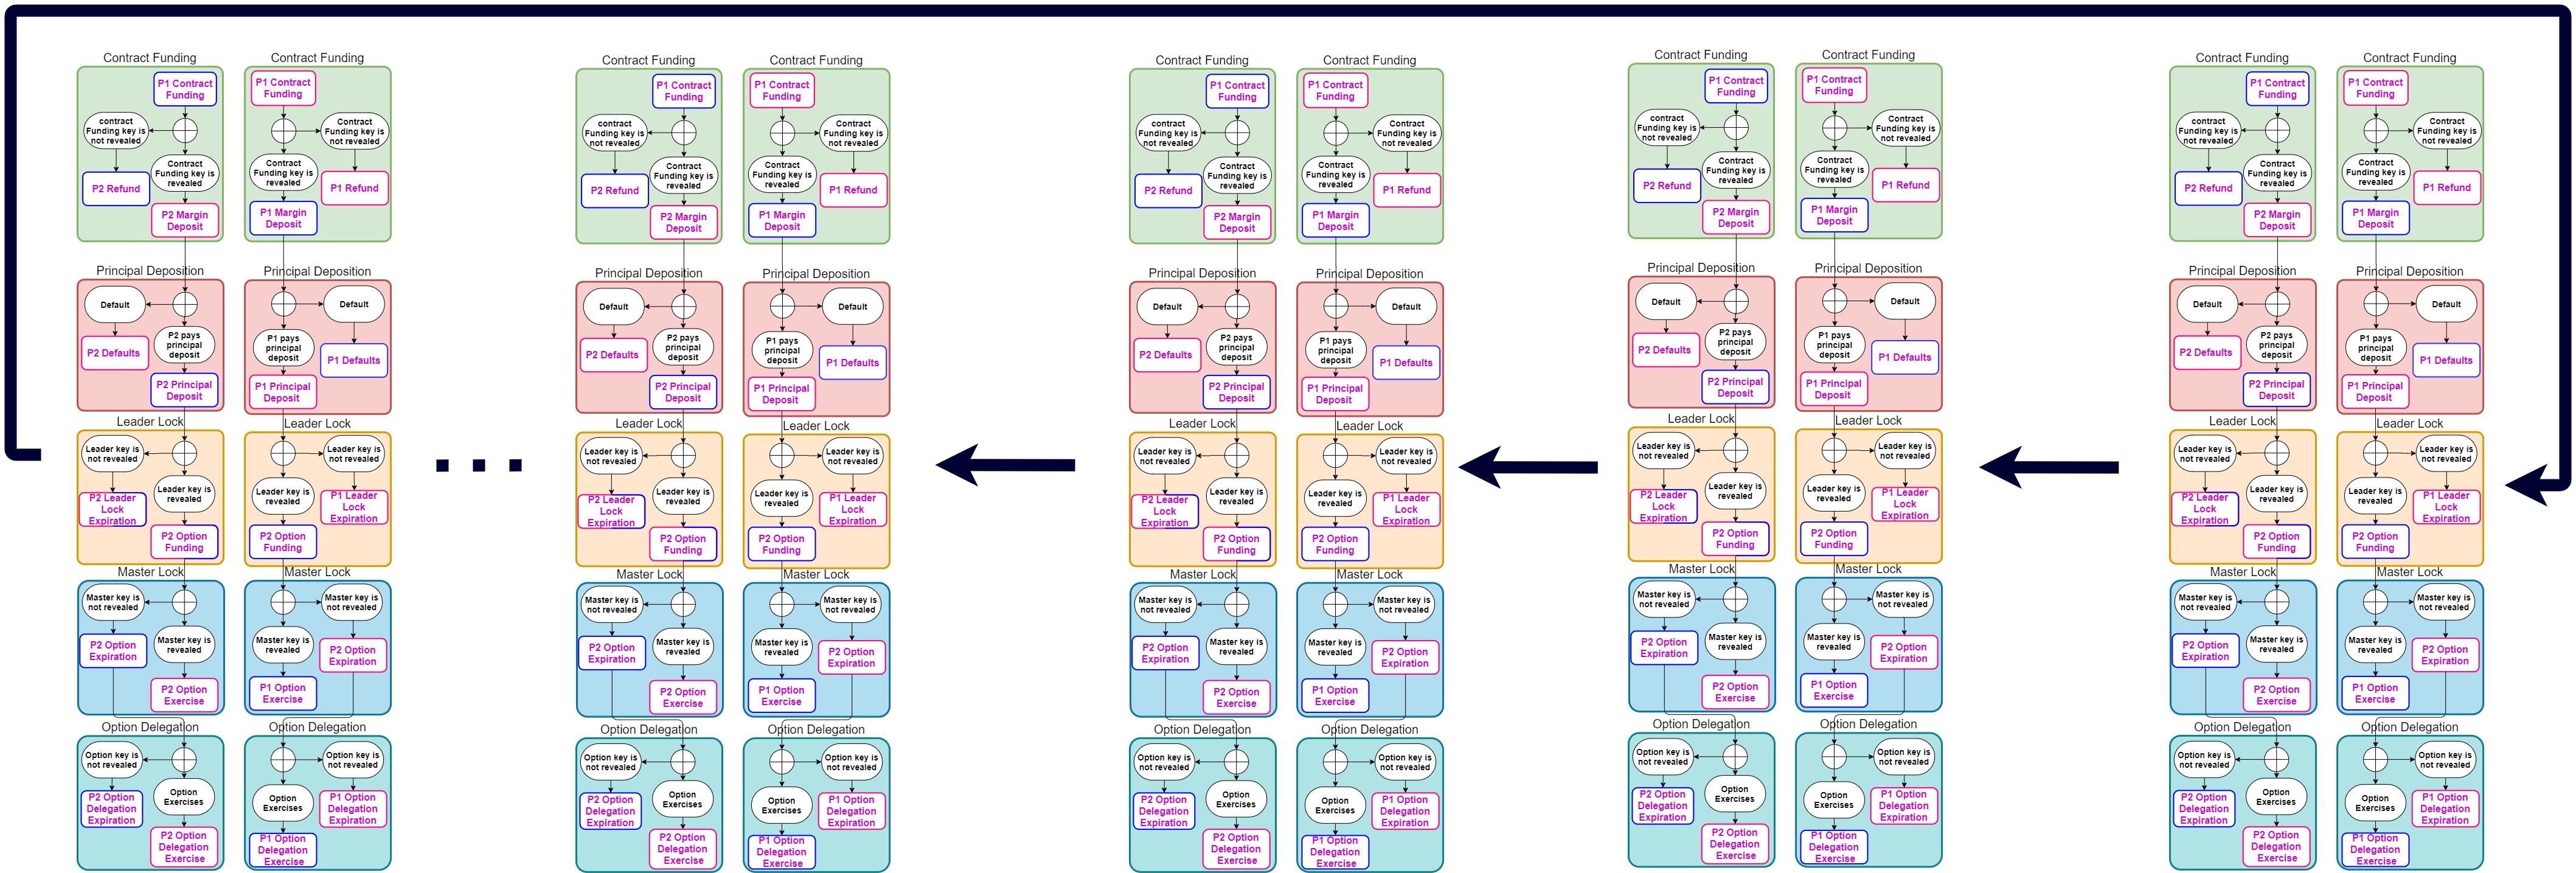
\includegraphics[width=\textwidth]{figures/looped arb.png}
    \caption{General form of the looped Arbitrage, composed of several instances of meta swaption.}
    \label{fig:meta_arb}
\end{figure*}

In this section we are going to elaborate on the term of arbitrage by redefining it in swaption market in the following way:
An arbitrage in the swaption market is an opportunity when a party, named exploiter, can exercise a chain of swaptions simultaneously, beginning from the exploiter's asset and also ending in the same asset, and profits by gaining more assets than the start point. Fig~\ref{fig:meta_arb} shows the general form of an arbitrage made up of several instances of \MetaSwaption forming a loop.

% \begin{definition}{\it Arbitrage Owner}
% In an arbitrage, the one who buys all the swaptions is called the Arbitrage Owner. In our examples she mostly is Alice. The Arbitrage Owner is also called the \Atwo Key Holder interchangeably.
% \end{definition}

We introduce four different types of arbitrages that are possible by adoption of our \MetaSwaption as their building blocks:
\begin{itemize}
    \item \textbf{Early deposition} arbitrage
    \item \textbf{Late deposition} arbitrage
    \item \textbf{Margin-free} arbitrage
    \item \textbf{Bonded} arbitrage
\end{itemize}


For further analysis, we give an example of arbitrage use cases. Alice, the exploiter whose initial asset is ACoin, is going to form an arbitrage making a chain of swaptions between Bob, Carol, Dave and Erin that take place concurrently. In section~\ref{sec:tangle} we will explain the procedure of signing contracts for each party in details but first we discuss about the general overview of our execution processes. For convenient reason, we index each swaption by order, \ie indexes of swaptions between Alice and Bob, and Alice and Carol, and Alice and Dave and Alice and Erin are respectively one to four.

Using the normal form of arbitrage shown in Fig.~\ref{fig:sep-arb}, the exploiter has to pay margin in every single swaption besides generating lots of transactions and thus, transaction fees. To solve this and to exercise the swaptions concurrently, we use the overlapping technique which changes the structure of our arbitrage model to Fig.~\ref{fig:overlap-arb}.

The overlapping technique is the action of extending the output's required signatures of all transactions to other parties in order to make additional guarantee.

\begin{figure}[htp]
    \caption{Arbitrage with and without overlapping technique}
    \subfloat[Arbitrage architecture using a loop of swaptions]{
    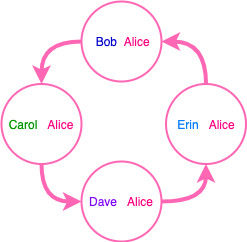
\includegraphics[width=0.45\textwidth]{figures/arb-sep.png}
    \label{fig:sep-arb}
  }~
  \subfloat[Arbitrage architecture using overlapping technique]{
  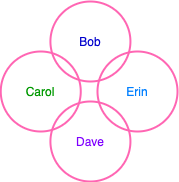
\includegraphics[width=0.45\textwidth]{figures/arb-overlap.png}
  \label{fig:overlap-arb}
  }
\end{figure}


% \begin{definition}{\it Genesis swaption}
% In an arbitrage, the swaption in which \Atwo key holder and \keyone key holder are faced together is called the Genesis Swaption. This swaption is supposed to be the first one processed in an arbitrage. 
% \end{definition}

%\subsection{Model}
% \subsection{Lined Arbitrage}
% \ahC{Are these lines in the good position?}

\subsection{Early Deposition Arbitrage}
\label{sec:line_arb}

Consider the following variation of our main example. Alice already has an amount of ACoin equal to the needed principal. First of all, she starts a swaption with Bob. After Bob deposits his principal, Alice can use his BCoins on her later swaption contracts. Then she trades these locked BCoins with Carol's CCoins, and these CCoins with Dave's DCoins and finally trades these DCoins with Erin's ACoins. According to the definition of arbitrage, now she has more ACoins than she primarily had. Since Alice primarily has enough ACoins, she only uses early deposition swpations. She technically can use a late deposition swaption for the first swaption, but since in that case she has to pay larger premium, it is not rational.
She also uses the swaption overlapping to transfer her assets between different swaption contracts. 
In Fig~\ref{fig:line_arb} this technique is shown. All parties share all transaction before any thing gets broadcast. After that, the procedure goes on as follows:

\begin{figure*}
    \centering
    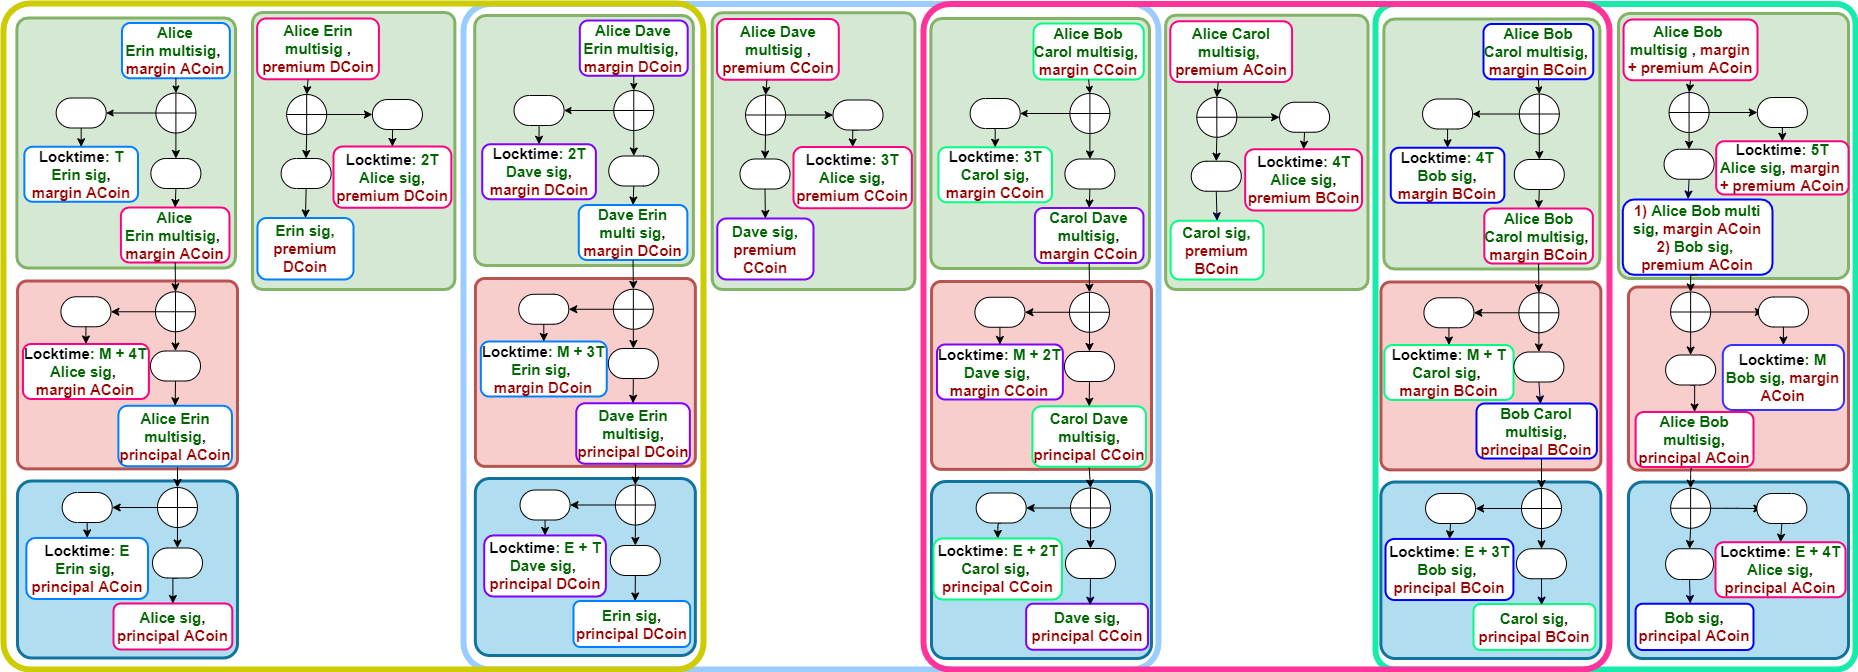
\includegraphics[width=\textwidth]{figures/arbitrage1-fateme.png}
    \caption{Example of an arbitrage, where Alice owns all ACoins primarily needed. On each transaction, signatures, output amount, and locktimes are specified. Pink-bordered transactions are broadcast by Alice, blue-bordered ones by Bob, green-bordered by Carol, purple-bordered by Dave and cyan-bordered by Erin. If there is a line between two transactions, then the source transaction is considered to be an input of the destination transaction.}
    \label{fig:line_arb}
\end{figure*}

\begin{itemize}
    \item \textbf{Contract funding}: Alice starts her contract with other parties simultaneously, by sharing the funding transaction with them. Then she decides whether to reveal \Aone key or not. If she does, all the swaptions go to the next stage. The locktimes are set descending from swaption number one to four, so that Alice can not cheat. In fact, Alice has to reveal \Aone before $T$, the minimum locktime among all swaptions, since otherwise at least one of them has expired and the entire arbitrage is not plausible any more. Note that if any of the funding stages fail, the entire arbitrage fails.
    
    \item \textbf{Principal deposition}: In this stage, every one has to deposit their principal. All swaptions are early deposition swaptions, so all the locktimes are ascending from swaption number one to four. Possible scenarios: 
    \begin{itemize}
        \item One of the parties defaults. In this case, all parties after the defaulter also default. Hence, the first defaulter looses his margin and all the other parties transfer their margin with the next party in the swaption with the next index and the last party transfers her margin to Alice.
        \item All parties deposit their principal and go to the next stage.
        
    \end{itemize}
    
    % \item \textbf{Leader Lock}:The locktimes in the first swaption are ascending and in the rest of swaptions are descending. The reason is that in the first one Bob holds the \keyone key and in other ones Alice holds it. Note that Bob has the M + P + 3T locktime but in fact he has to reveal \keyone key before M + P, because otherwise Alice defaults and Bob loses his margin. parties take back their own money. By arranging timelocks in this way, no portion of parties can cheat on others by cooperating. Possible scenarios:
    
    % \begin{itemize}
    %     \item Bob defaults. he looses one of his margins as discussed in {\it Late Deposition} swaption, while other
    %     \item Bob reveals \keyone key by broadcasting Alice's option funding transaction. Then Alice broadcasts the Erin's Option Funding transaction, and other opponents do the same respectively. And we go to next stage. If any of them does not do this, the only one who looses money is that party.
    % \end{itemize}
    % \ahC{is it clear and okay or not? We can mention that all of the swaptions in the point of view of other opponent than Alice is just like an instance of Meta Swaption, accordingly no body can cheat by cooperation on others}
    
    \item \textbf{Option funding}: It is time for Alice to use her option. She reveals \Atwo key for Erin, then each party reveals it for the previous one in order. Therefore, the locktimes are descending in all swaptions from swaption number one to four.
\end{itemize}

\subsection{Late Deposition Arbitrage}
\label{sec:margined_arb}
% \subsubsection{Margined Arbitrage}
Now, consider the case that Alice does not own enough ACoin to start such a procedure. She has to pay ACoin to Bob using a portion of ACoins she gets from Erin. This would only be possible if she had the ability to spend Bob's BCoins and do all the tradings with it and finally deposit the ACoins taken form Erin to the first swaption. To do so, she can use the late deposition swaption as the first swaption. We call it the late deposition arbitrage. Fig.~\ref{fig:margined_arb} depicts such an arbitrage. There are four swaptions, and Alice pays only premium in all of them. She also has to deposit margin in the first swaption. Alice's margin is only there to prevent her from cheating due to the cyclic locktimes on the funding stages (in the next section we will briefly explain this problem and our proposed solution). Therefore, there are five margins and four swaptions. The first swaption to start is the same as the last swaption to finish and it is actually between Erin and Bob (swaption number one). The five phases of late deposition arbitrage are: 

\begin{figure*}
    \centering
    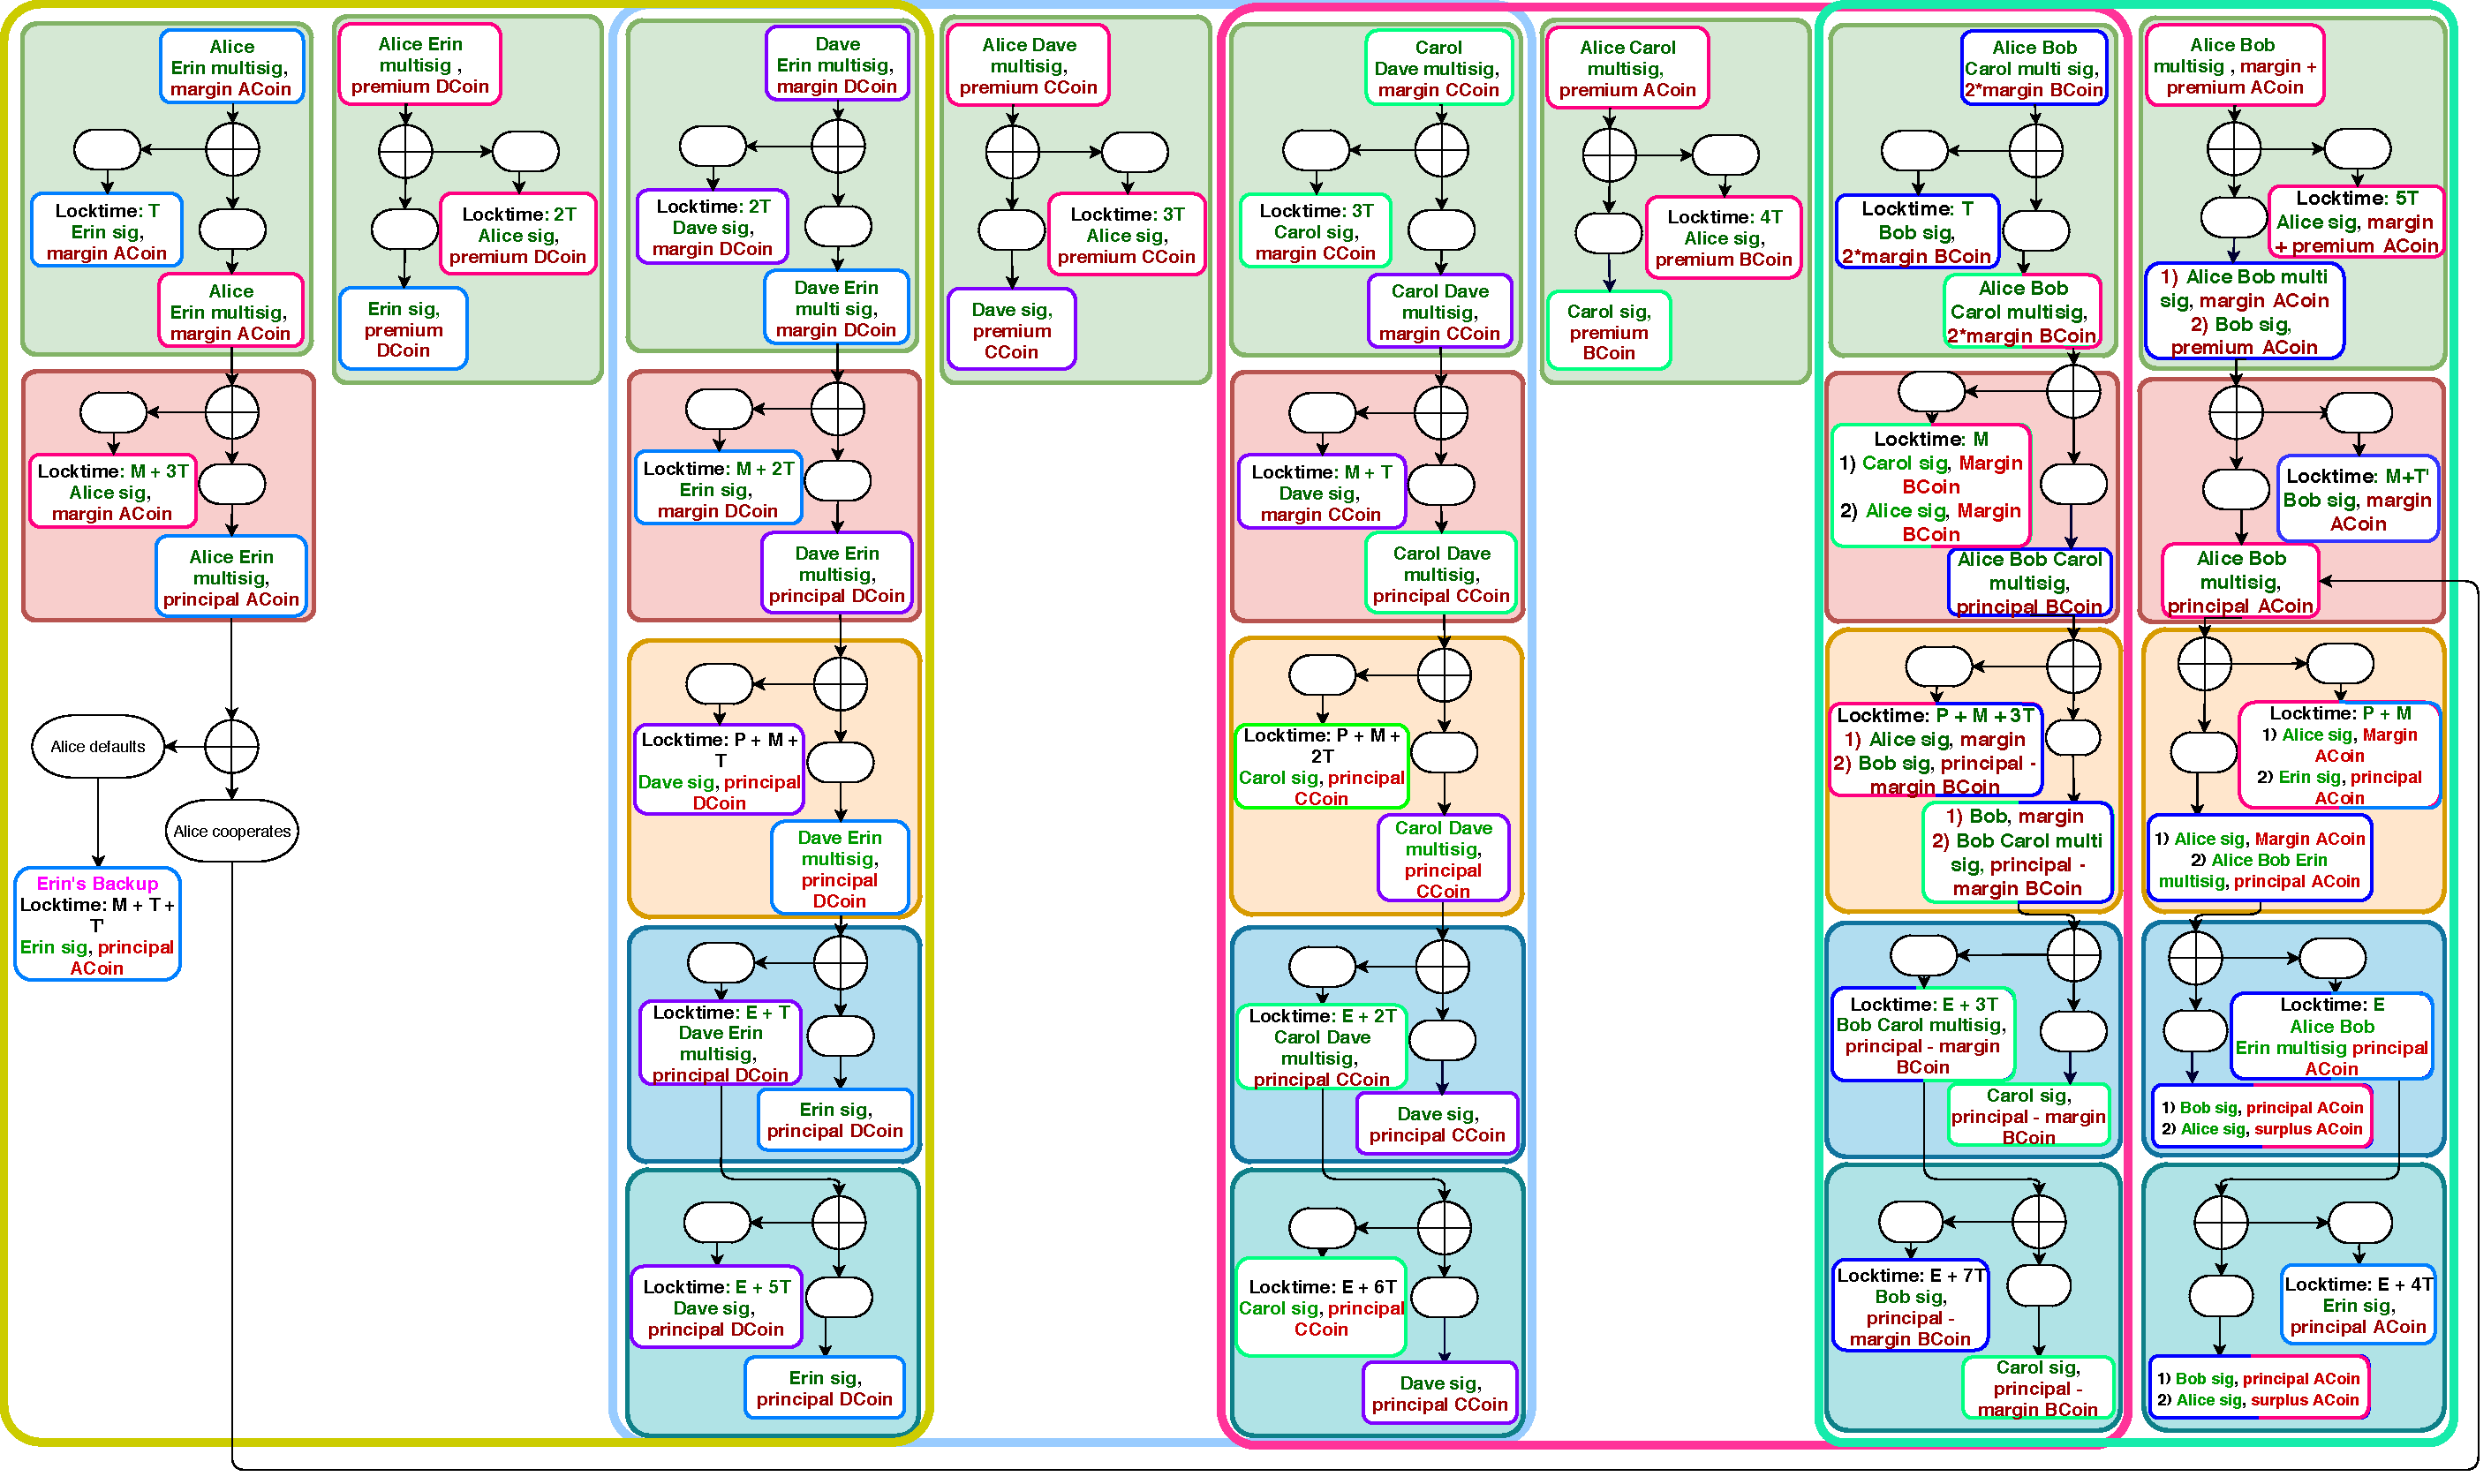
\includegraphics[width=\textwidth]{figures/arbitrage-late.pdf}
    \caption{The schematic for late deposition arbitrage. The transactions with two border colors, can be broadcasted with both corresponding parties.}
    \label{fig:margined_arb}
\end{figure*}


\begin{itemize}
    \item \textbf{Contract Funding}: Similar to the early deposition arbitrage, every one has exchanged funding and refund transactions. Three types of these stages:
    \begin{itemize}
        \item Alice's first funding includes margin + premium.
        \item Other fundings of Alice only include premium.
        \item Bob's funding includes margin and an amount of guarantee. Here the amount of guarantee is equal to the margin, so Bob's funding is worth twice other parties margins.
        \item Other parties fundings include only margin.
    \end{itemize}
    Alice reveals the \Aone key by broadcasting Erin's margin deposit transaction. Then, Erin broadcasts Dave's margin deposit transaction and everyone broadcasts the margin deposit transaction of their previous party. No one has the incentive not to broadcast this transaction since if she does not, she is the only one who goes through a loss. When all the margin deposit transactions are broadcast, the arbitrage proceeds to the next stage.
    
    \item \textbf{Principal deposition}: All swaptions except for the first one are early deposition, so the locktimes of principal deposition on these swaptions are ascending from swaption number two to four. On the other hand, the first swaption is late deposition, so Alice's locktime has to be greater than Bob's. Alice's principal is in fact a portion of the principal that Erin deposits. Similar to the early deposition arbitrage, if any one defaults in this stage, and does not deposit his principal, the faulty party loses his margin (except for when it is Alice that exchanges her margin with Bob's) and other parties margins are exchanged with their previous party. As mentioned earlier, the first swaption is in fact between Erin and Bob, but Alice also puts margin to this swaption. The principal deposition of Erin is an any-one-can-pay transaction. The amount of $M+T'$ needs to be greater than $M+3T$, hence if Erin defaults, Alice can default too. If Erin does not default and broadcasts her principal deposition transaction, Alice takes its output as an input to the principal deposition of the first swaption. We have given Erin a chance that if Alice does not do so, she can take her principal back and of course since Alice has defaulted, she exchanges her margin with Bob's. If everyone deposits their principal, we go to the next stage.
    % \ahC{Revise the entire paragraph}
    \item \textbf{Leader lock}: Alice is waiting for Bob to reveal the \keyone key by broadcasting the Erin's option funding transaction on first swaption. If Bob does so, Erin broadcasts Dave's option funding transaction and every other party broadcasts the previous party's option funding transaction respectively. Locktime for Alice is the shortest and increased from swaption number four to two and for Bob is the longest. Bob's option funding transaction can be broadcasted by both Carol and Bob. Otherwise, other parties can collude and cheat on Bob using the following attack: Bob reveals the \keyone key and others do not broadcast the Bob's option funding and take Bob's margin. Hence, when Bob can broadcast his own option funding, there would not be any problem of this kind. 
    
    Thus, if Bob reveals the key, every other party goes to the next stage. If Bob does not reveal, he loses his margin. If Bob reveals the \keyone key after $P + M$, Alice will take back her margin and immediately reveal the \Atwo key which results in taking Bob's money in both swaptions, thus discouraging Bob from delaying in exposure. 

    \item \textbf{Option funding}: This is the time for Alice to use her option. She can reveal the \Atwo key by broadcasting the Erin's option exercise. She takes her surplus and Bob gets his ACoins. She has to reveal it within $E$ locktime. Since in all swpations the buyer party,
    \ie right-hand side party, is in charge of revealing the \Atwo key, the locktimes have to be descending. This means the locktime of the Erin's option expiration transaction has to be both longer and shorter than the Bob's option expiration. This is obviously impossible. Hence, we set the locktimes so that Carol's locktime is longer than Alice's, which makes it possible for Carol and Alice to cheat on Bob, but we solve this problem using the delegation stage. Now, if Alice exercises her option until $E$ locktime, then every party can take their new coins. If Alice does not exercise until $E$, her option is delegated to Bob.
    
    \item \textbf{Option delegation}: If Alice has not exercised until $E$, Bob broadcasts the Erin's option expiration and Bob's option expiration transactions and all other parties do the same (since it is their only chance to get their coins). The arbitrage is now in the delegation stage. Bob has the option and everyone is waiting for him. If he decides to exercise, everyone gets their new coins, otherwise everyone gets their former coins. The locktimes are descending for all swaptions except for the first one which is ascending (like last stages), since now Bob is the key holder of this stage and he is in charge of revealing the \Delegation key. 
    % \fatemeC{The most important consideration is that if Alice has decided not to exercise her option, Bob would also not exercise. Since if it was not beneficial for Alice it would not be beneficial for Bob neither. the reason is that the coins that Alice gets are the same as Bob gets, so if one has lost its value the other one has lost too.(why the hell????)}
 
\end{itemize}
\begin{figure*}
    \centering
    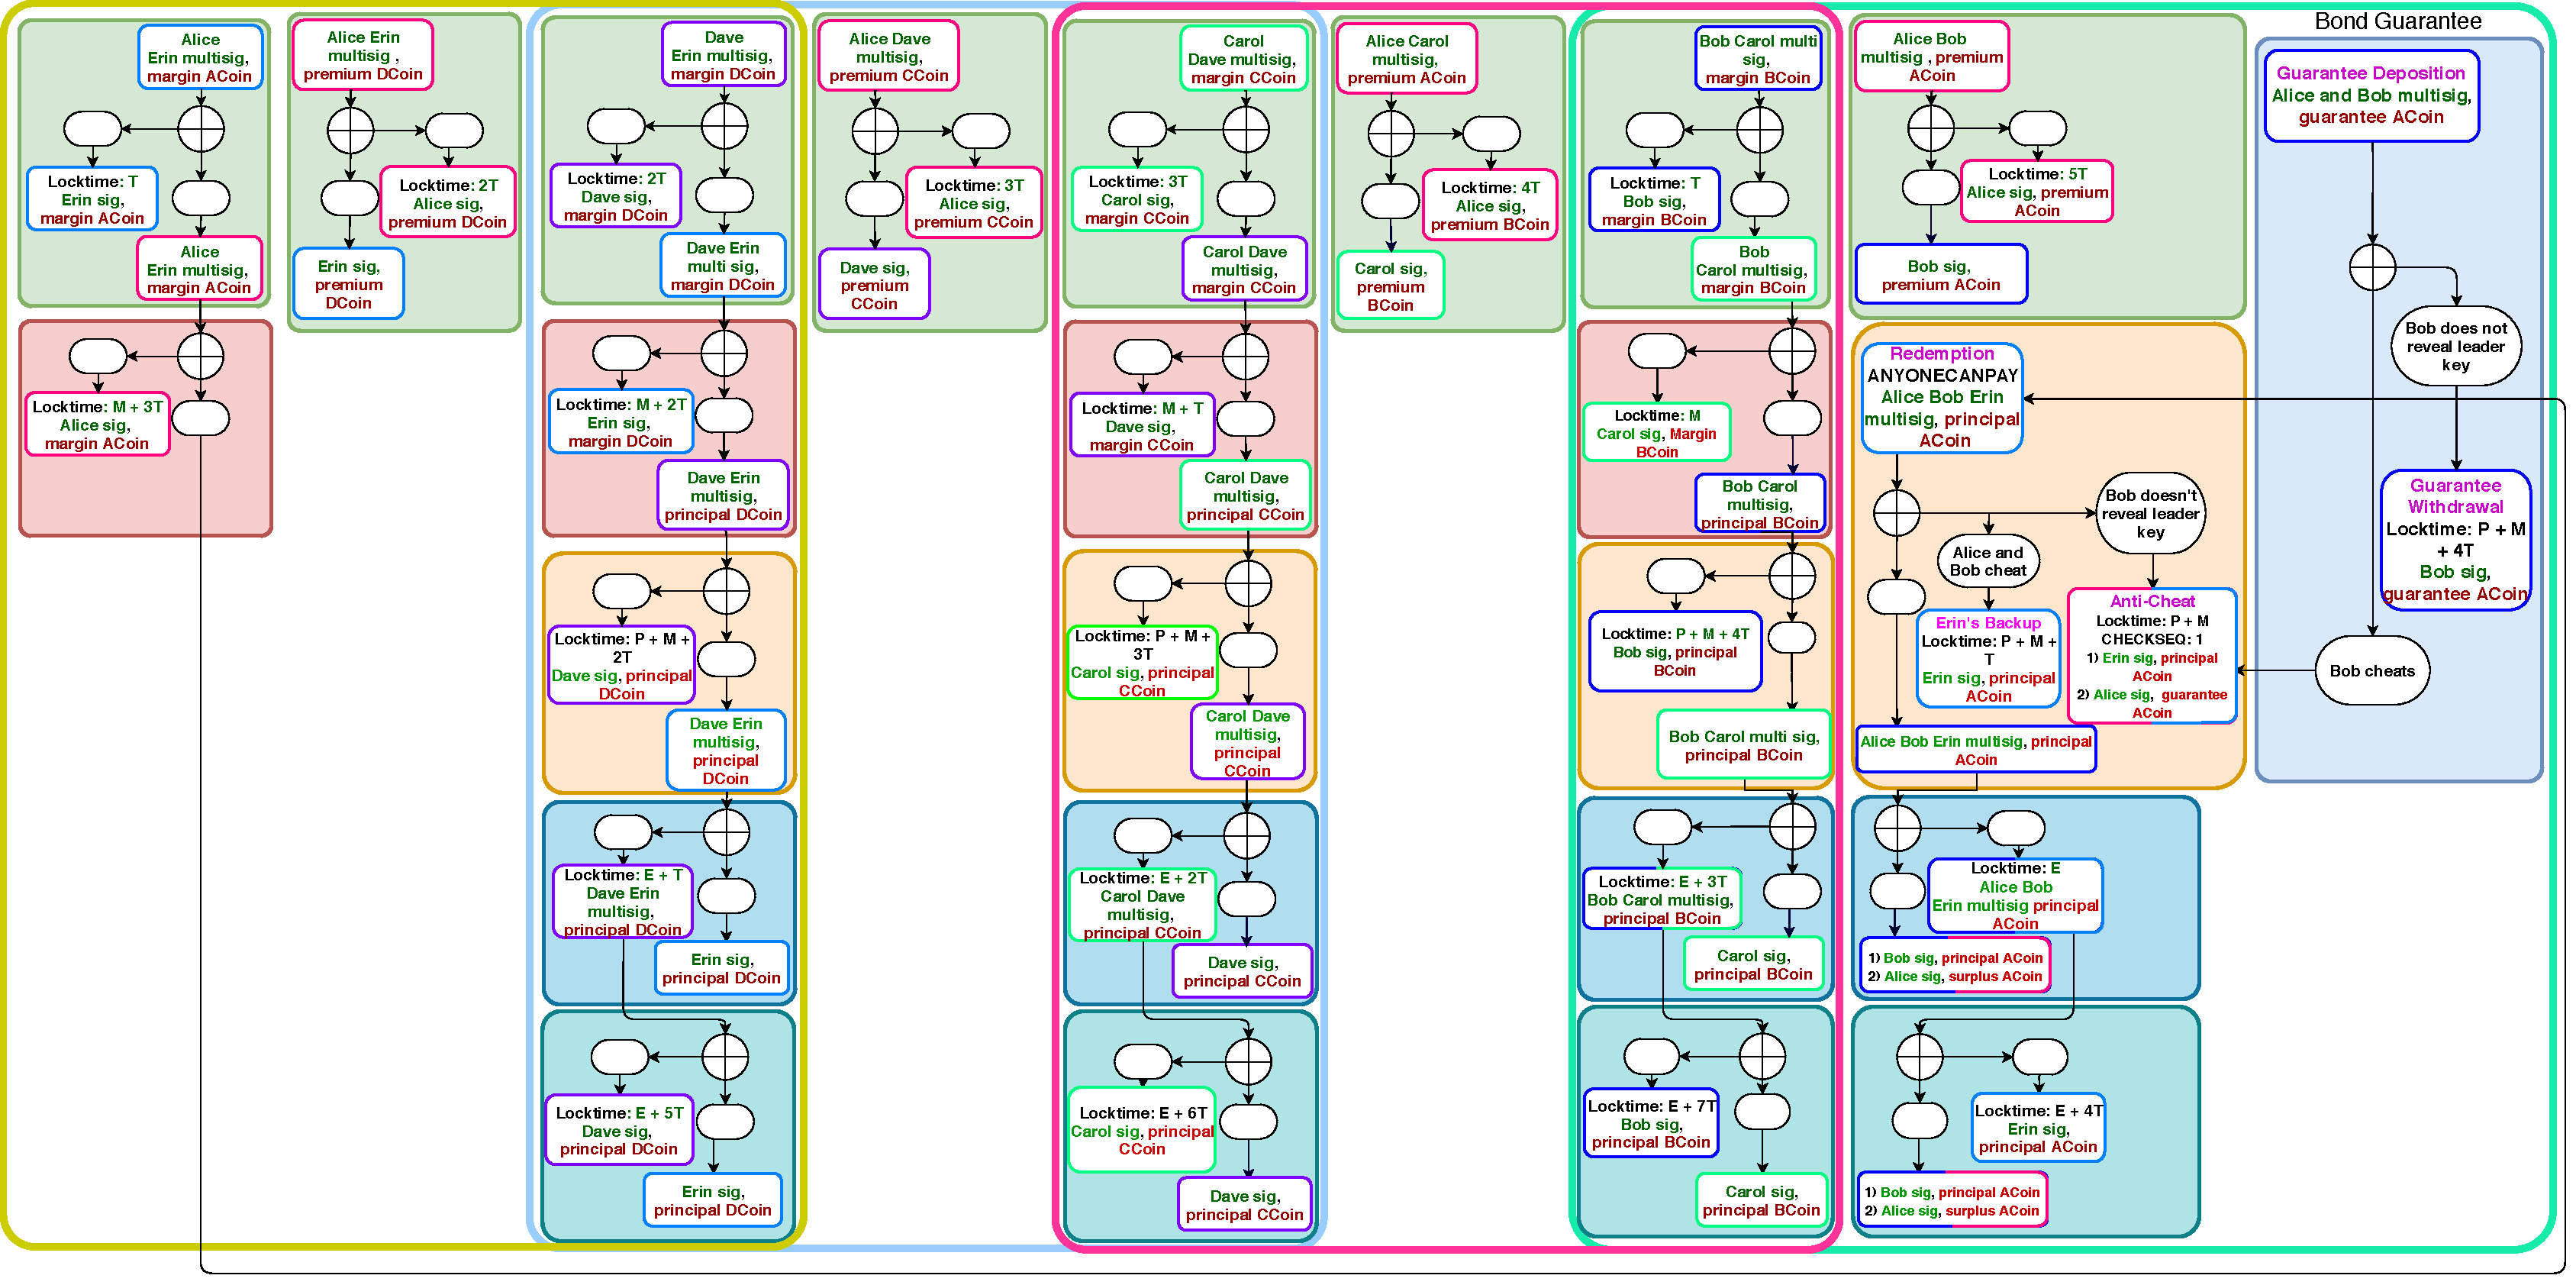
\includegraphics[width=\textwidth]{figures/arbitrage-bonded.pdf}
    \caption{The bonded arbitrage using ABCD.}
    \label{fig:abcd-arb}
\end{figure*}

\subsection{Margin-Free Arbitrage}
%\vspace{-1mm} 
Next, we are going to study the case in which Alice does not have enough ACoin for margin deposition in her swaption with Bob but still she can afford the minimal amount of ACoin as guarantee besides all the premiums. Using the margin-free swaption mentioned in previous section, an arbitrage can be built and exploited satisfying our need. Before all, we have to analyse the amount of guarantee in a margin-free swaption. If this type of swaption is used lonely without further contracts, the minimum valuable amount is enough for the amount of guarantee (even if it is less than premium). However, to use it alongside other contracts, \eg~as the first swaption in an arbitrage setting, Alice needs to set the guarantee value of Bob more than the summation of all the premiums which she wants to spend in her later contracts. Otherwise, Bob is incentivized to pretend himself as the other parties in later contracts, \eg~in our example Carol or Dave or Erin, and cheats on Alice by stealing Alice's premiums in the later swaptions by not exposing the \keyone key and loosing his guarantee. Note that if Bob acts honestly, the guarantees in both sides will be exchanged. In fact, assume the amount of margin is worth $m$ times more than the amount of premium. The margin-free swaption can be used, if the number of parallel swaptions, is less than $m$. Otherwise, it is better to use a late deposition swaption instead. We do not include the figure for margin-free arbitrage, however, it is simply derivable from previous arguments.

\subsection{Bonded Arbitrage}
For final case, we suppose that Alice even does not have enough money for guarantee needs in a margin-free swaption. Alice still can make an arbitrage using the ABCD component devised in previous works, as her first swaption \cite{tefagh2020atomic}. In this way, she does not need more money than the premiums for her arbitrage. We call this type of arbitrage, the bonded arbitrage, since the arbitrage exploiter bonds her initial asset in the first place. The bonded arbitrage is shown in Fig.~\ref{fig:abcd-arb}.
% \ahC{The figure is ABD, we need an ABCD one}

\begin{table*}[]
    \centering
    \begin{tabular}{|c|c|c|c|}
    \hline
        {\normalsize Stage} & {\normalsize LT in column $1$} & {\normalsize LT in column $2i$} & {\normalsize column $2i + 1$}\\
        \hline
        
        {\normalsize Contract Funding} &
        {\normalsize $(N + 1)T$} &
        {\normalsize $(N - i + 1)T$} &
        {\normalsize $(N - i + 1)T$} \\
        
        {\normalsize Principal Deposition} &
        {\normalsize $M + T'$} &
        {\normalsize $M + (N - i)T$} & - \\
        
        {\normalsize Leader Lock} & {\normalsize $P + M$} &
        {\normalsize $P + M + iT$} & - \\
        
        {\normalsize Option Contract} & 
        {\normalsize $E$} &
        {\normalsize $E + (N - i)T$} & - \\
        
        {\normalsize Option Delegation} & 
        {\normalsize $E + NT$} & 
        {\normalsize $E + (2N - i)T$} & - \\
        \hline
    \end{tabular}
    \caption{Locktimes for general case in an arbitrage. Each column in the table shows one column in the arbitrage.}
    \label{tab:arb}
\end{table*}

Now, consider the general case for the arbitrage when there are $N$ swaptions.
Table \ref{tab:arb} shows locktimes for each stage in a general arbitrage. Each column in the table shows one column in the arbitrage. Moreover, for simplicity we put locktimes so that different stages do not have overlap in time. In some cases overlapping stages can cause trouble. Two examples are: 

\begin{itemize}
    \item $M$ has to be larger than $(N + 1)T$. Otherwise, Alice and Carol can broadcast the Bob defaults transaction and then broadcast the Alice's refund and take Bob's margins.
    
    \item In the third stage, $P + (N - 1)T$ has to be greater than $T'$. Otherwise, Alice can wait untill $P + M + (N - 1)T$ not depositing principal, then Bob has to broadcast the Bob's leader key expiration and then Alice will deposit and then broadcast the Alice's leader key expiration. So, she takes Bob's margin without loosing anything but premium.
\end{itemize}

Note that Alice in fact has $E$ time to use her option. Then Bob takes the option, so we can say that Alice does not have any option but it is not true for two reasons: 1) Arbitrages are always zero-risk. 2) If she deposits her principal it means that all the parties have cooperated (if one does not, she does not deposit principal and does not lose anything, just the margins are exchanged which is inevitable). When all parties have cooperated and arbitrage is zero-risk every thing is fine so why would Alice not exercise?

Note that in such cases Alice is always going to use her option, so Alice is not in fact delegating her option to Bob, but by having the delegation stage, she only assures Bob that he would not be cheated.
%\ahC{koja tozih dadim ke delegation mitone bejaie oon method e maskhareie Atomic Cross-chain Swap estefade beshe?}

% \ahC{Time Elapsed Experiment.}\\
% \ahC{Reconstruction impossibility}\\
% \fatemeC{Is it reasonable to remove Option parts from Arbitrage. Arbitrages have absolute benefit in a short time, so the option is not needed to be given to Alice. However she can have it by adding the rest of the transactions.}\\
\section{Tangled Money Market}
\label{sec:tangle}

\begin{figure*}
    \centering
    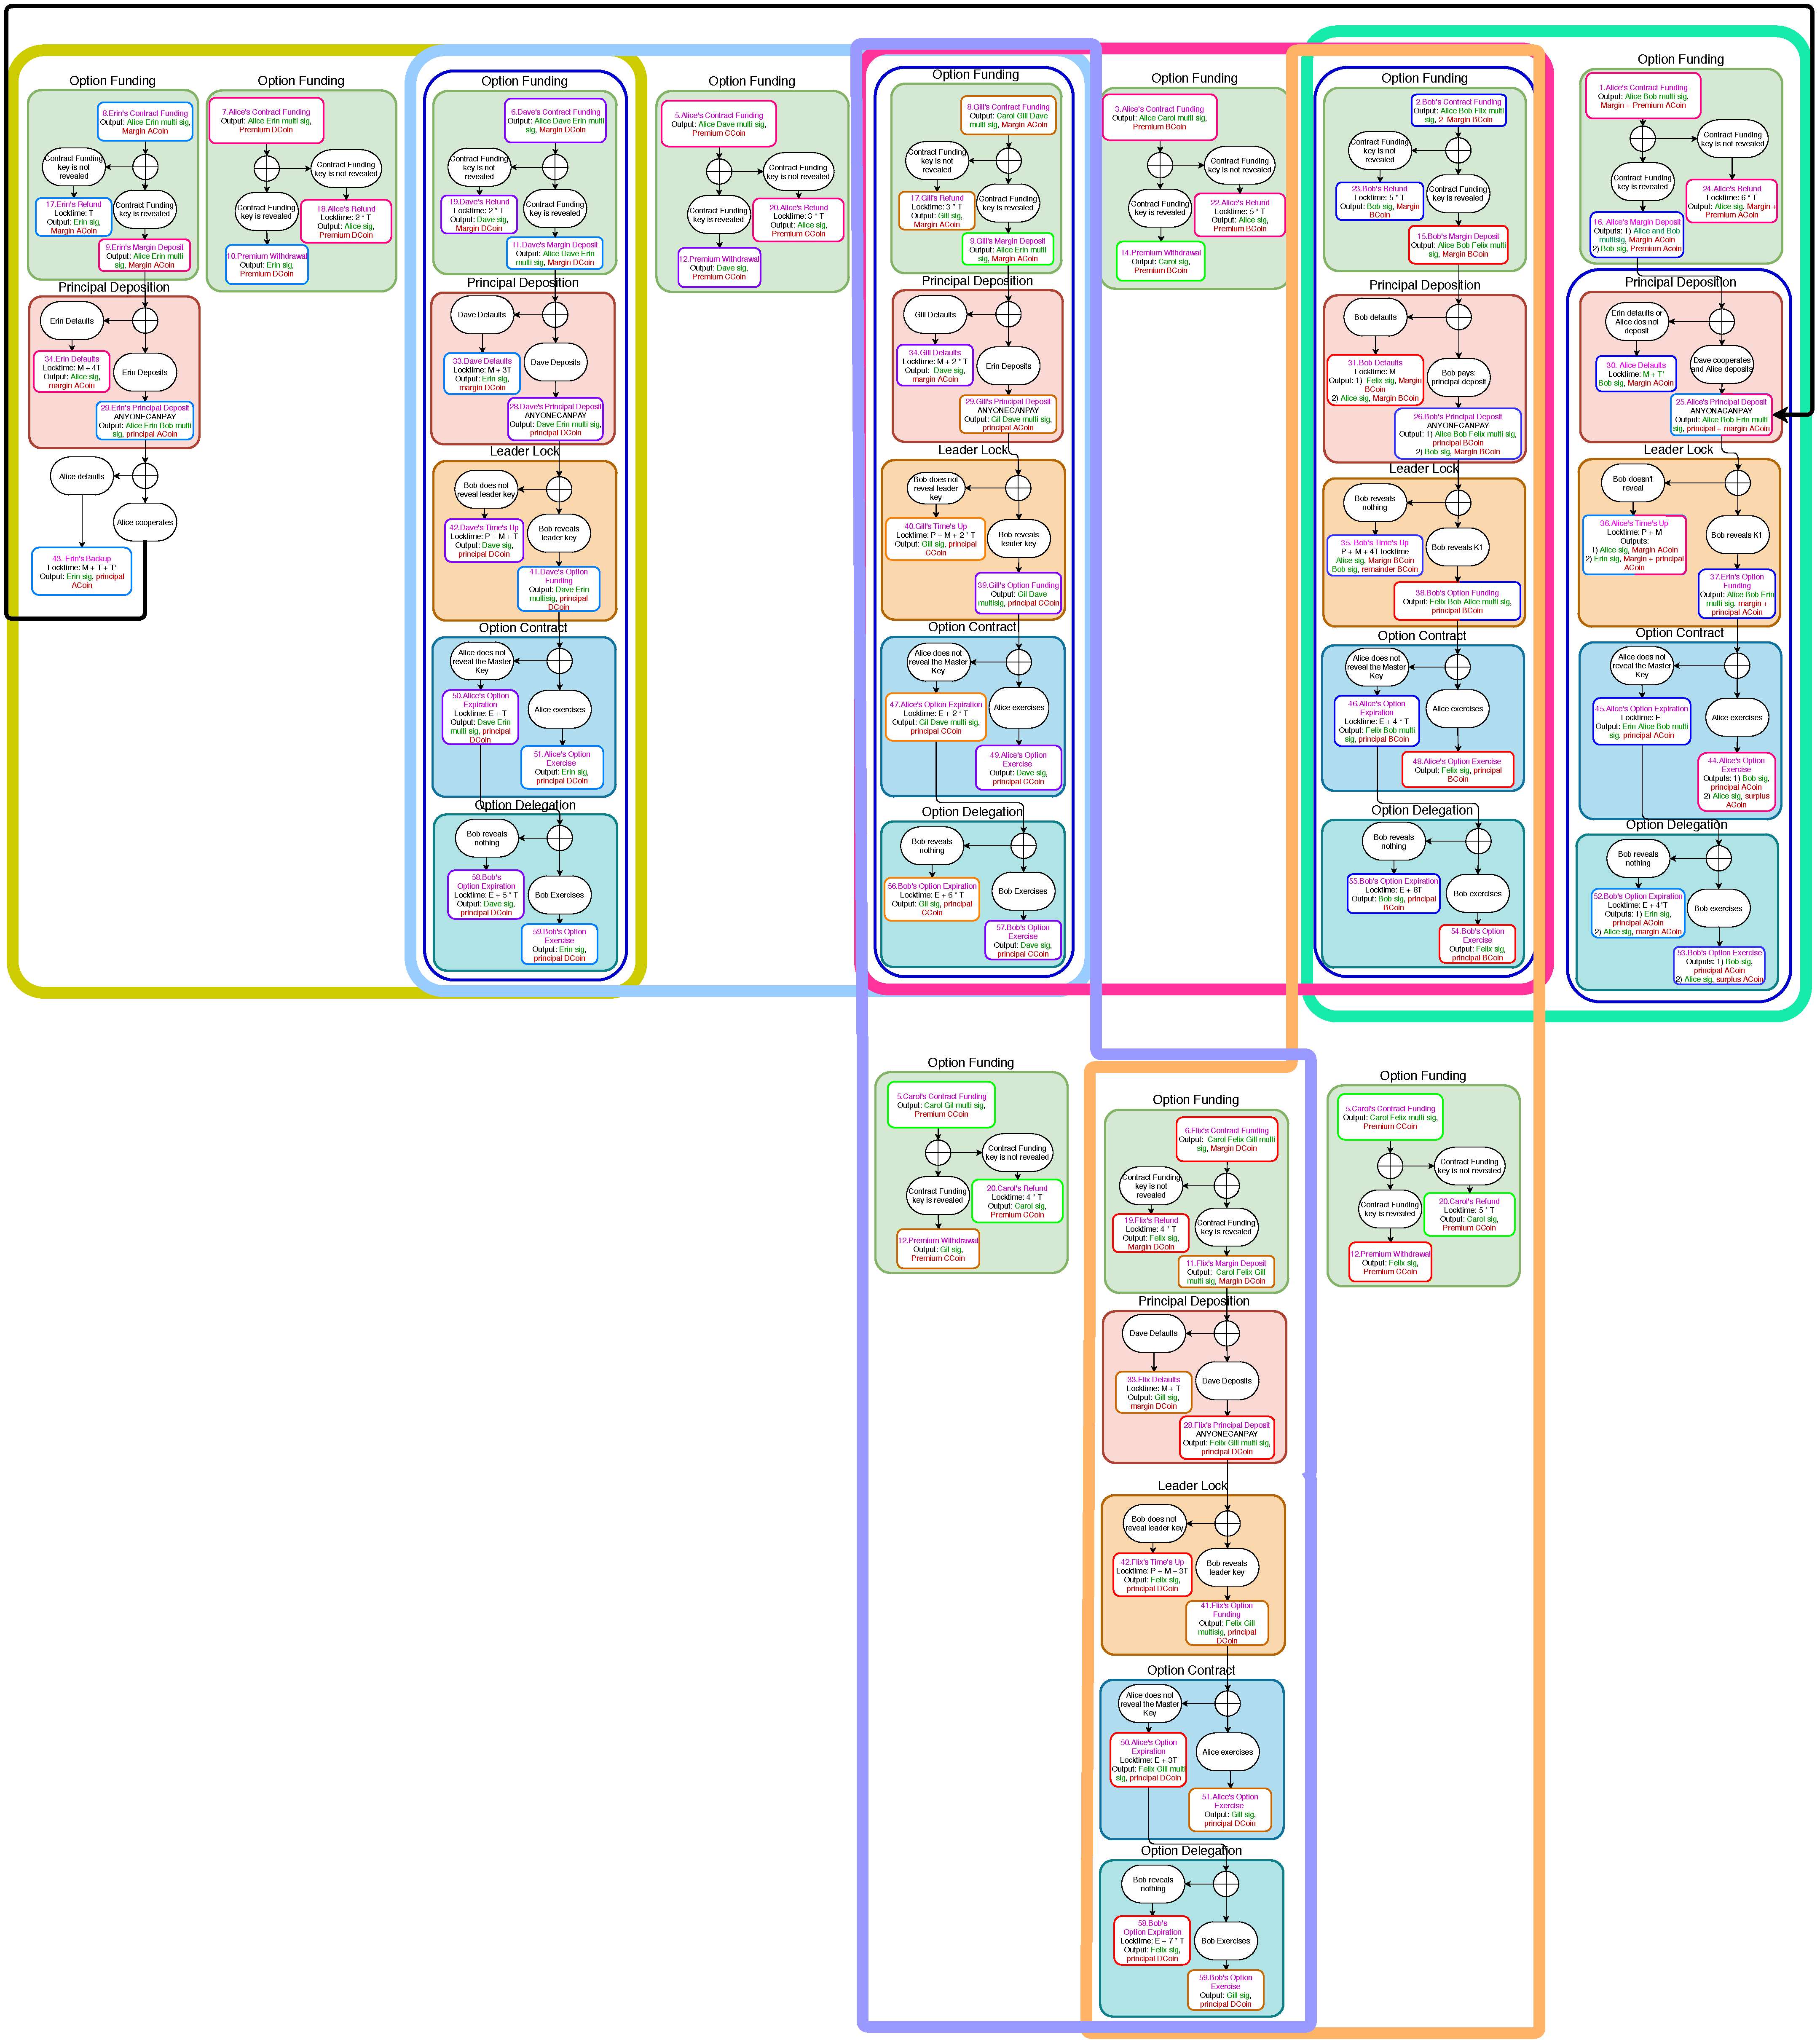
\includegraphics[
    width=\textwidth,
    ]{figures/tangle.pdf}
    \caption{a tangle of two arbitrage loops; one for Alice and one for Carol}
    \label{fig:tangel}
\end{figure*}

So far, we have studied an arbitrage with one exploiter and all other parties only as sellers. Now, imagine each of the sellers can be an exploiter in a second arbitrage using the principal from the first arbitrage. We call such intertwined arbitrages as tangled money market whose example is shown in Fig.~\ref{fig:tangel}. Furthermore, these tangled swaptions do not have to be in the form of arbitrage. In other words, a series of swaptions entangled together is counted as a tangled money market. In this section, we prove two theorems for tangles. And by designing a protocol we provide a constructive proof for our final theorem.

Note each transaction may have multiple inputs and outputs in real word. We only consider those transaction involved in a tangle have single input and output. 
% inputs and outputs whose both source and destination transactions are involved in the tangle.
We define $P=\{p_1,\ ,p_2,\ ..,\ p_n\}$ as the set of distinct parties which are participating in the tangle even through different accounts.

First of all, to analyse a tangle we introduce two graph models:

\begin{enumerate}
    \item Swaptions graph: $\mathcal{G}_s=(V, E)$ where $V$ is the finite set of vertices each representing a swaption, and $E$ the finite set of edges. Each edge is an ordered pair of vertices. In a set of overlapping swaptions, each swaption is shared between three parties $p_1, p_2, p_3$, where $p_1$ is the buyer of the swaption. In order to build the $\mathcal{G}_s$, each of these swaptions is shown as two separate swaptions; one between $p_1$ and $p_2$, and the other one between $p_1$ and $p_3$. This is another interpretation of the overlapping process. Where in real world, $p_1$ is an intermediary who mediates between $p_2$ and $p_3$, in this interpretation, she actually takes $p_2$'s principal to deposit in the swaption between herself and $p_3$. For each vertex $v \in V$ there are two functions $\beta: V \to P$ and $\sigma: V \to P$ which indicate the swaption buyer and seller respectively. Each edge represents transfer of principal between two swaptions. An example of this graph is shown in Fig.~\ref{fig:gen-graph}.

    
    \item Principal flow graph: This graph represents the flow of principal and \keyone key. $\mathcal{G}_{p} = (V_p,E_p)$ where $V_p$ is the finite set of vertices and $E_p$ the finite set of edges.
    For each swaption in $\mathcal{G}_s$ there are two vertices in $V_p$ corresponding to it. Each of them represents a party in the swaption. The function $\ell(v)$ where $\ell(v): V_p \to P$ returns the party related to vertex $v$. Each $e \in E_p$ is an ordered pair of vertices $(h(e), \tau(e))$ that $h(e)$ and $\tau(e) \in V_p$. For the above example there would be four vertices with labels $p_1, p_2, p_1$ and $p_3$. Clearly, there is a correspondence between each vertex of $\mathcal{G}_s$ to a pair of vertices in $\mathcal{G}_{p}$. We define the function $\rho: E_p \to \{i, x, t\}$, such that the following properties hold:
    \begin{itemize}
        \item For each $e \in E_p$ that $\rho(e) = i$, $e$ connects two vertices of one swaption and represents the deposition order inside a swaption \ie $h(e)$ has to deposit earlier than $\tau(e)$ by the locktime rules. Note that for each $v \in V_p$, there is a unique $e \in E_p$ such that $v$ is either $h(e)$ or $\tau(e)$, since each vertex is participating in a single swaption. We define function $\mathcal{O}: V_p \to V_p$ where for a vertex $v, \mathcal{O}(v)$ is the other vertex connected to the unique edge $\Tilde{e}$ with $\rho(\Tilde{e}) = i$ connected to $v$.
        
        \item For each $e \in E_p$ that $\rho(e)=x$, $e$ represents the flow of principal between swaptions i.e. the principal moves from $h(e)$ to $\tau(e)$. We also define successor and precursor of a vertex as the functions $s: V_p \to V_p  \cup \O $ and $p: V_p \to V_p \cup \O$ such that for each $v \in V_p$ if there is $e \in E_p$ that $\rho(e)=x$ and $h(e)=\mathcal{O}(v)$ then $s(v)=\tau(e)$ and if there is no such $e$ then $s(v)=\O$ and for each $v, u \in V_p$ if $s(v)$ is $u$ than $p(u)$ is $v$ and if there  is no $v \in V_p$ such that $s(v)$ is $u$, then $p(u)$ is $\O$. Functions $s$ and $p$ are well-defined since there can not be any two edges $v$ and $u$ with $\rho(v) = \rho(u)= x$ such that $h(u) = h(v)$ or $\tau(u) = \tau(v)$. As an intuition, given our previous example, the successor of $p_1$'s vertex corresponding to the swaption with $p_2$ is his vertex corresponding to the swaption with $p_3$, and the precurser of $p_1$'s vertex corresponding to his swaption with $p_3$ is his vertex correspondingo the swaption with $p_2$.
        
        The $\mathcal{G}_{p}$ graph of previous example is shown in Fig.~\ref{fig:prin-flow-graph}. It is clear that for each $v \in V_p$, $\ell(s(v)) = \ell(v)$, since otherwise the party $\ell(v)$ transfers his asset to party $\ell(s(v))$ without getting anything back, which is not rational. With the same argument, $\ell(p(v))$ is equal to $\ell(v)$. We call this, the rationality property of $\mathcal{G}_{p}$.
        
        \item Consider all $v \in V_p$ that there is no edge $e \in E_p$ that $\rho(e) = x$ and $\tau(e) = v$. Then, for each $i \in \mathbb{N}$ that $\mathcal{O}(s^i(v)) \neq \O$, there is an edge $e'$ that $\rho(e') = t$ and $\tau(e') = v$ and $h(e') = \mathcal{O}(s^i(v))$. This type of edge, will later be used to impose a deposition order between two vertices in two adjacent swaptions in order to guarantee the safety of parties who inject principals to the system rather than transform it from another swaption.
        
        % \ahC{Definition has to be if and only if, but I don't know how}
        
        % if $\rho(e)=t$, then there is an $i \in \mathbb{N}$ that $h(e) = \mathcal{O}(s^{i}(\tau(e)))$ and there is no $b \in E$ that $\rho(b)=x$ and $\tau(b)=\tau(e)$.
        % \melikaC{I don't understand! yani in poolaro bayad az jib avorde bashe, na in ke ba ye edge e x i avorde bashe}
    \end{itemize}
    % See Fig.~\ref{fig:prin-flow-graph}.

It is worth mentioning that in $\mathcal{G}_{p}$ there is no cycle $c$ that for all of its edges $e$  $\rho(e) = x$, since otherwise the principal transferred through $c$ would not have any sources.

\end{enumerate}



\begin{figure}
    \centering
    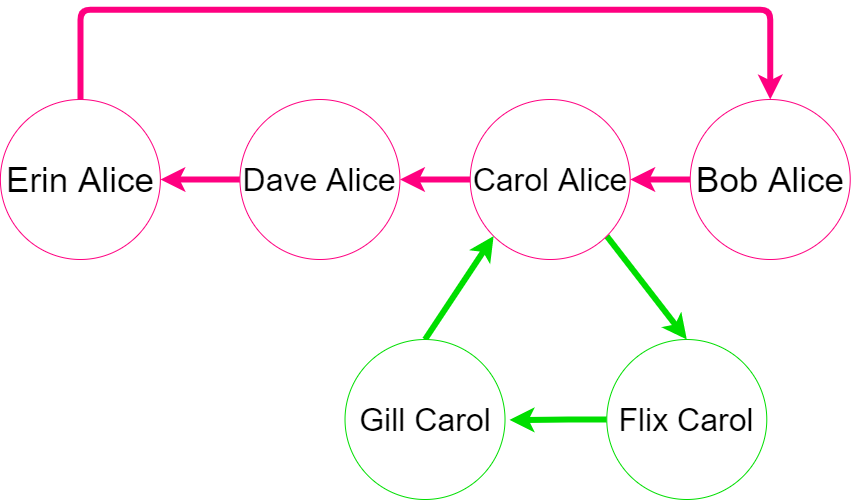
\includegraphics[width=0.7\textwidth]{figures/gen-graph.png}
    \caption{Example for \genGraph graph}
    \label{fig:gen-graph}
\end{figure}

\begin{figure}
    \centering
    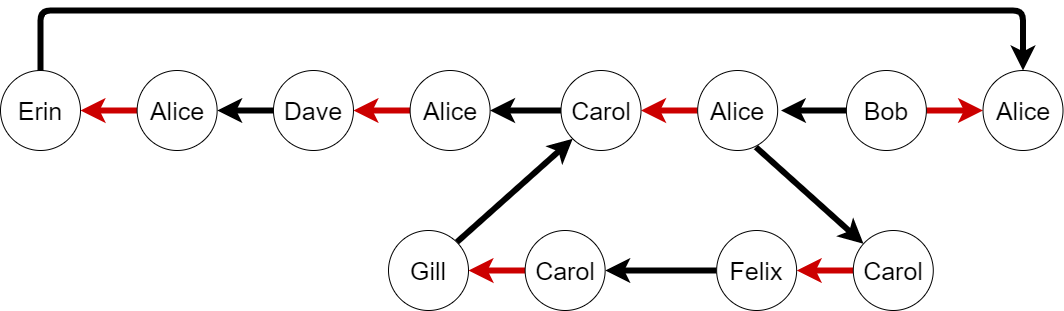
\includegraphics[width=\textwidth]{figures/prin-flow-graph.png}
    \caption{Example for $\mathcal{G}_{p}$ graph}
    \label{fig:prin-flow-graph}
\end{figure}

% \begin{figure}
%     \centering
%     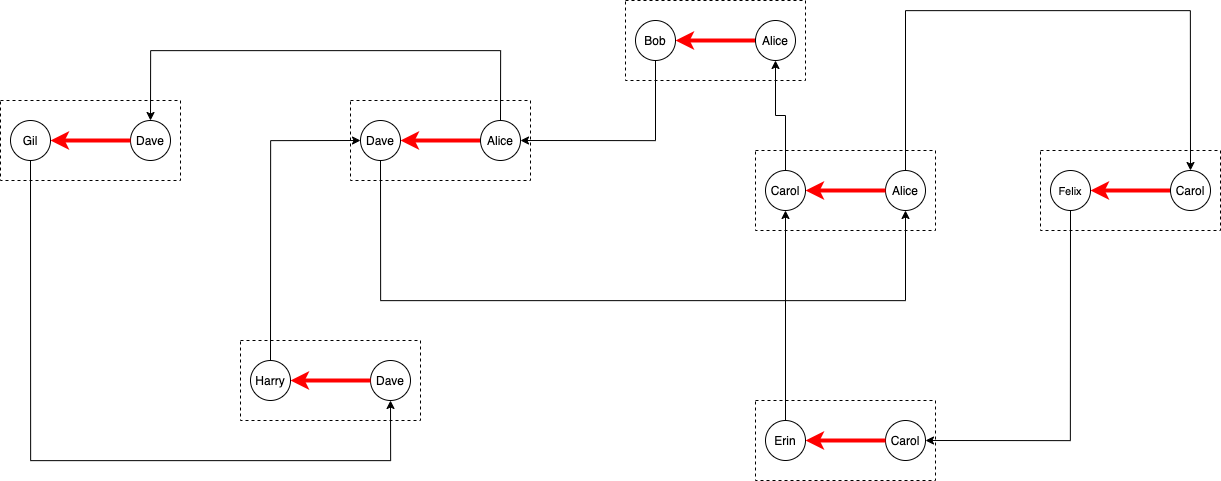
\includegraphics[width=\textwidth]{figures/lock-imposition-graph.png}
%     \caption{Example for \AtwoGraph Graph}
%     \label{fig:lock-impos-graph}
% \end{figure}


\begin{definition}{\it Concurrent Tangle}\\
A tangle $T$ is concurrent if the \genGraph graph representing $T$ is a \scdg.
\end{definition}


\begin{definition}{ Association Set}\\
In the $\mathcal{G}_s$ graph, a vertex $v$ is in the association set of party $p_i$ if $\beta(v) = p_i$ or $\sigma(v) = p_i$.

\end{definition}

For later usage, we need to find the $p_{master}$ for a tangle.
Given a \genGraph graph $\mathcal{G}_s=(V, E)$ of a tangle $T$, we design a graph $\mathcal{G}_{r}=(V_r,E_r)$ such that $V_r=\mathcal{P}$ and for every $v \in V$ there is an edge $\hat{e} \in E_r$ for which $h(\hat{e}) = \beta(v)$ and $\tau(\hat{e}) = \sigma(v)$. Each vertex of $\mathcal{G}_{r}$ from which all the vertices are reachable \cite{bang2008digraphs} is a candidate whose label is eligible to be the $p_{master}$ of $T$.
% Note that strongly connected property of swaptions graph of $T$ is neccessary (not enough) condition to find an eligible $p_{master}$ for $T$. Therefore, if 
% \begin{algorithmm}
% {\it Owner Finder}
% \label{algo:owner-finder}
% \\
% \end{algorithmm}
% \begin{algorithm}
% \caption{Master finder}
% \begin{algorithmic}
% \State $\mathcal{C}=\mathcal{P}$
% \For{$i$ \textbf{from} $0$ \textbf{to} $n$}
%     \For{$j$ \textbf{from} $0$ \textbf{to} $n$}
%         \If {there is no path from $v_i$ to $v_j$ in $\mathcal{G}_{t}$}
%             \State remove $p_i$ from $\mathcal{C}$
%             \State break
%         \EndIf
%       \EndFor
%     % \State add $p_i$ to $\mathcal{C}$
%  \EndFor
%  \State return $\mathcal{C}$
% \end{algorithmic}
% \end{algorithm}



% The output of the algorithm is the list of candidate labels which are eligible to be the $p_{master}$ of $T$. 

% A tangle $T$ is \AtwoOk if the algorithm~\ref{algo:owner-finder} outputs at least one candidate party. 

For every graph $\mathcal{G}_1=(V_1, E_1)$, according to the definition of {\it feedback edge set} previously stated in \cite{bondy2000graph}, given $L$ the feedback edge set of $\mathcal{G}_1$ that $L \subseteq E_1$, the edge-induced subgraph $\mathcal{G}_2=(V_2, E_2)$ of $\mathcal{G}_1$ that $V_2=V_1$ and $E_2=E_1-L$ is acyclic.

\begin{definition}{\it Protected}\\
\label{def:pfok}
Assume subgraph $\mathcal{G}_{t}=(V', E')$ of $\mathcal{G}_{p}$ where $V'=V_p$ and $E'=\{e \in E_p | \rho(e) \neq t\}$.
A tangle $T$ is \keyoneOk if
\begin{enumerate}
    % \item $\mathcal{G}_{t}$ has only one source. We call this source, the \depsrc of $T$ and assume $\ell(\depsrc) = p_{leader}$.
    \item For all the source\footnote{A vertex $v$ in the graph such that there is no edge $e$ that $\tau(e) = v$} vertices $v$ in $\mathcal{G}_{t}$, $\ell(v)$ has to be identical and we assume $\ell(v)=p_{leader}$.
    \item $\mathcal{G}_{p}$ has a feedback edge set $L=\{e_0, e_1, ..e_l\}$ that for all $e_i \in L$, $\ell(\tau(e_i))= p_{leader}$ and $\rho(e_i) \in \{i, t\}$. 
\end{enumerate}

\end{definition}

 
% As it is clear, if the tangle is \keyoneGraph acceptable, then its $\mathcal{G}_{pf}$ graph has no more than one source. Since the $\mathcal{G}_{pf}$ graph has more edges than its $SG$ subgraph. \fatemeC{maybe should move it}

% \ahC{How can we explain the exceptional cases in which two keyone holder randomly choose the same key, or by cooperating?}


\begin{definition}{\it Cooperable}\\
A concurrent tangle $T$ is cooperable if it is \keyoneOk and there is at least one party eligible to be its $p_{master}$.
% algorithm~\ref{algo:owner-finder} outputs at least one candidate party when executes on $T$.
\end{definition}


% For each concurrent tangle, we call the output party of algorithm~\ref{algo:owner-finder}, the \Atwo key holder of $T$.

Now, we provide an example for a cooperable tangle. Fig.~\ref{fig:example-swp} shows the \genGraph graph, and Fig.~\ref{fig:example-pf} represents the principal flow graph of this example. All the source vertices in the principal flow graph have the label $B$, thus the party $B$ is $p_{leader}$. The principal flow graph has a feedback edge set with all the edges pointing to $B$'s vertices. Additionally, the Fig.~\ref{fig:example-gr} shows the $\mathcal{G}_{r}$ in which there is a path from vertex $A$ to every other vertex. Therefore, the party $A$ is the $p_{master}$ of this concurrent tangle.
% the property mentioned in protected definition.  
% Fig.~\ref{fig:example-pf} shows the principal flow graph of a cooperable tangle.

\begin{figure}
    \centering
    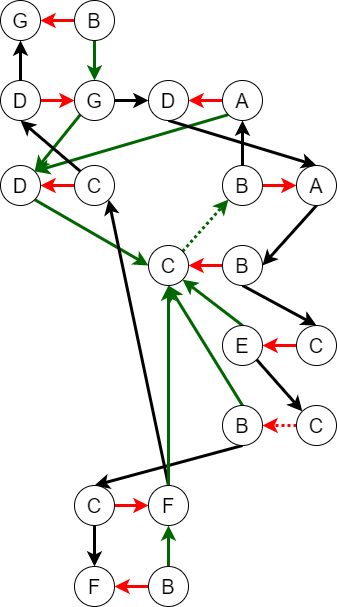
\includegraphics[width=0.8\textwidth]{figures/example.png}
    \caption{Principal flow graph of a cooperable tangle. Green, red and black edges represent edges whose $\rho$ function is equal to $t, x$ and $i$ respectively. Dotted edges are the feedback edge set of the graph.}
    \label{fig:example-pf}
\end{figure}
\begin{figure}
    \centering
    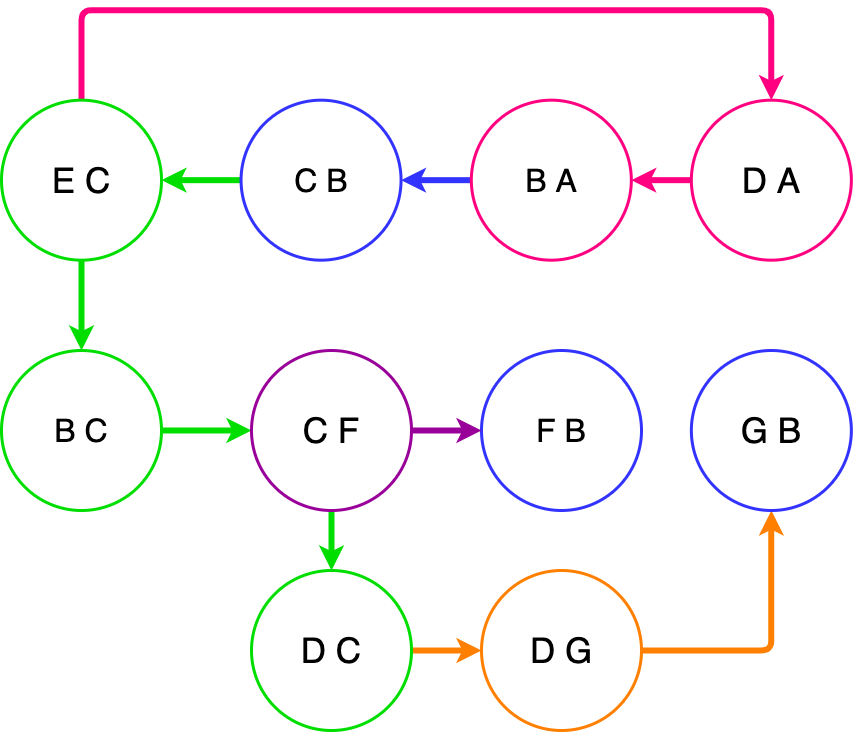
\includegraphics[width=0.5\textwidth]{figures/cooperable-example-swaption.png}
    \caption{Swaptions graph of a cooperable tangle. A node with the colors pink, blue, green, purple, and orange represents a swaption whose buyer is A, B, C, F, and G, respectively. The color of each edge represents the party who is transmitting the principal.}
    \label{fig:example-swp}
\end{figure}
\begin{figure}
    \centering
    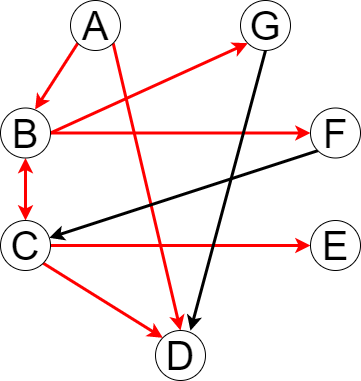
\includegraphics[width=0.5\textwidth]{figures/cooperable-example-tour.png}
    \caption{The $\mathcal{G}_{r}$ graph for our example to find the party $p_{master}$. Red edges show that the parties $B, C, D, E, F, $ and $G$ are reachable from party $A$.
}
    \label{fig:example-gr}
\end{figure}
Before delving into the first theorem, we need to define the required security property for executing such a tangle. To do so, we define multiple classes for the future of every distinct parties in the tangle. We assume that for a fix desired party, every other party can act cooperatively for cheating on him.

% \begin{figure}
%     \centering
%     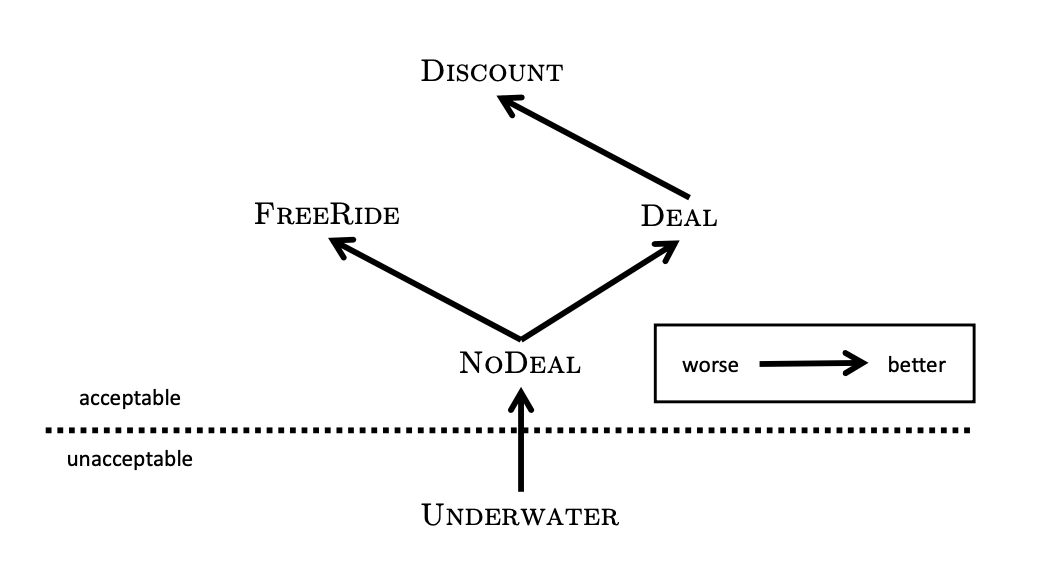
\includegraphics[width=\textwidth]{figures/outcomes.png}
%     \caption{The priority of feasible state in the point of view of each parties.}
%     \label{fig:outcomes}
% \end{figure}

To be consistent with prior terminology first introduced by Herlihy in his paper ``Atomic Cross-Chain Swaps", for a party $p_i$ we define these states \cite{herlihy2018atomic}:

\begin{itemize}
    \item Nodeal: There is no swaption in $p_i$'s {\it associated set}, that has been executed. Hence, he keeps his prior assets without getting any new assets.

    \item Deal: The swaptions in $p_i$'s association set are all properly executed and the amount of principals inside them are finally swapped.

    % \ahC{\item Discount: In at least one of swaptions in $p_i$'s association set, $p_i$ does not pay his principal while acquires other party's principal or premium and in all its other swaptions the principals are swapped completely.}

    \item Freeride: The party $p_i$ does not pay anything through the entire tangle while getting some asset as premium or principal at the end of execution phase.

    \item Underwater: In at least one swaption, he does not gain any new principal, while he loses his principal.

\end{itemize}
Now we can properly give a definition of the needed security property for our tangle: 
A protocol $P$ for a tangle $T$ is secure if after execution of $P$ on $T$, none of the parties who have adhered to $P$ enter the underwater state.
Next, it is time to state the first theorem:
\begin{theorem}
\label{th:concurrency}
For every cooperable tangle $T$, there is a secure protocol $P$.

\end{theorem}
% \begin{figure}[htp]

%     \caption{The conceivable shapes of a sink node. The blue dashed-line arc is optional.}
%     \subfloat[Form 1]{
%     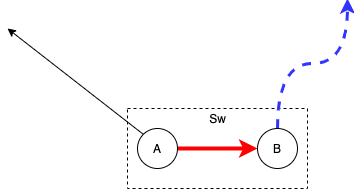
\includegraphics[width=0.45\textwidth]{figures/sink-node-2.png}
%     \label{fig:sink-1}
%   }~
%   \subfloat[Form 2]{
%   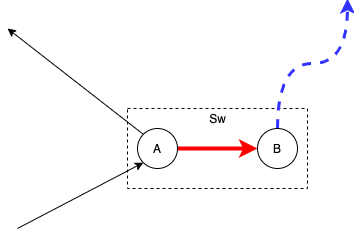
\includegraphics[width=0.45\textwidth]{figures/sink-node-4.png}
%   \label{fig:sink-2}
%   }
%   \label{fig:sink-shapes}
% \end{figure}
% \begin{figure}
%     \centering
%     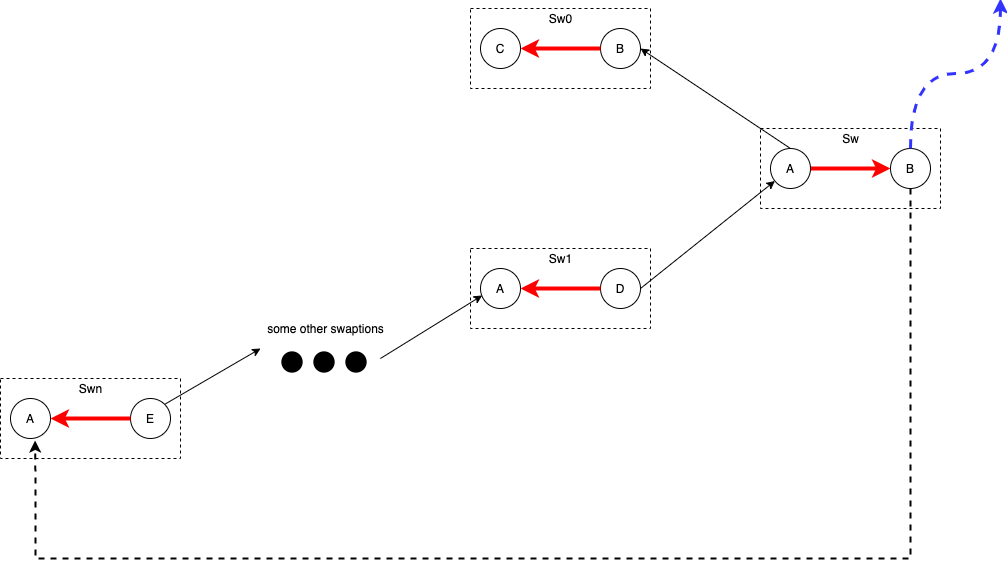
\includegraphics[width=\textwidth]{figures/sink-node-1.png}
%     \caption{The sink node which is the end of a line.}
%     \label{fig:sink-3}
% \end{figure}
% \begin{figure}
%     \centering
%     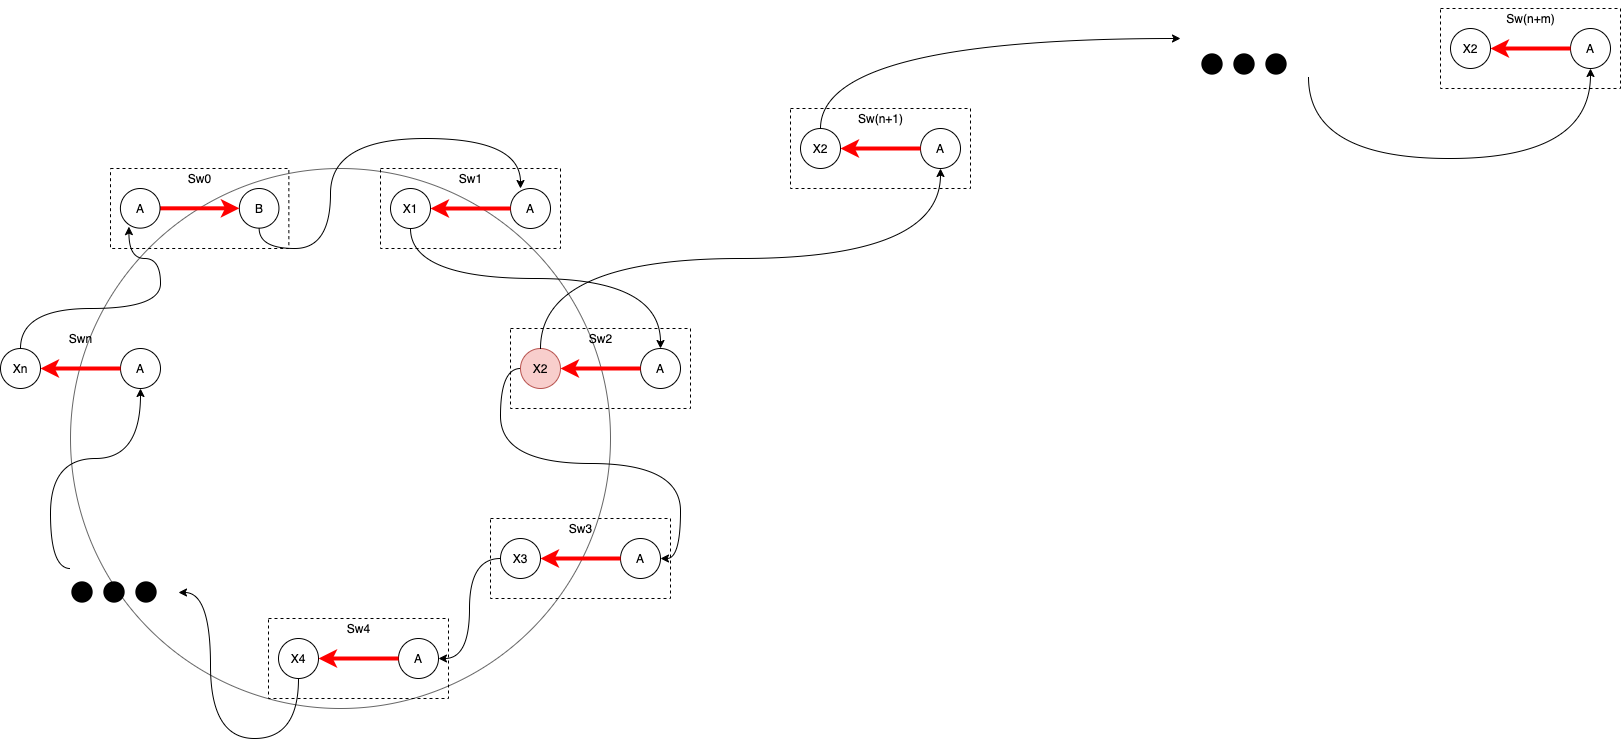
\includegraphics[width=\textwidth]{figures/sink-node-3.png}
%     \caption{The looped sink node.}
%     \label{fig:sink-4}
% \end{figure}
\begin{lemma}
\label{lm:sink}
In the edge-induced subgraph $\mathcal{G}_k=(V_k, E_k)$ of $\mathcal{G}_{p}=(V_p, E_p)$ of the concurrent \keyoneOk tangle $T$, that $V_k = V_p$ and 
% edges $e \in E$ that $\tau(e) = p_{leader}$ and $\rho(e) \in \{i, t\}$ are removed in $E'$,
$E_k = E_p - \{e \in E_p \ |\ \tau(e) = p_{leader}, \rho(e) \neq x \}$, for each sink\footnote{A vertex $v$ in the graph such that there is no edge $e$ that $h(e) = v$} vertex $s$, $\ell(\mathcal{O}(s)) = p_{leader}$.

\end{lemma}
\begin{proof}
We prove the above lemma by contradiction. Assume there is a sink vertex $s \in V_k$ that $\ell(\mathcal{O}(s)) \neq p_{leader}$. 

Firstly, for the vertex $\mathcal{O}(s)$ there must exist an edge $e \in E_k$ such that $\rho(e)=x$ and $h(e)=\mathcal{O}(s)$, since otherwise the vertex in $\mathcal{G}_s$ corresponding to $s$ would have no output edge and thus the $\mathcal{G}_{s}$ would not be strongly connected.

Secondly, there must exist an edge $e' \in E_p$ that $\tau(e')=\mathcal{O}(s)$ and $\rho(e')=x$, since otherwise the vertex $\mathcal{O}(s)$ would be one of the source vertices of $\mathcal{G}_{t}$ graph defined in the definition~\ref{def:pfok}. Then, according to definition~\ref{def:pfok}, $\ell(\mathcal{O}(s)) = p_{leader}$ which contradicts the assumption. 

Thirdly, in $\mathcal{G}_k$, there must exist an edge $\tilde{e} \in E_k$ which $\rho(\tilde{e})=i$ and $\tau(\tilde{e}) = s$. Since if $s = h(\tilde{e})$, this would contradict the assumption of $s$ being a sink. On the other hand, as mentioned before, in $\mathcal{G}_{p}$ there is a unique $\tilde{e}$ which $\rho(\tilde{e})=i$ connected to each vertex. So if there is no $\tilde{e} \in E_k$ that $\rho(\tilde{e})=i$, this unique edge would be a member of $E_p - E_k$ and would
have been removed in $\mathcal{G}_k$. According to the definition of $\mathcal{G}_k$, this means that $\ell(\mathcal{O}(s)) = p_{leader}$ which contradicts the assumption.

Finally, we know that $p(\mathcal{O}(s)) = \mathcal{O}(h(e'))$. Now, in $\mathcal{g}_k$, if there is $i > 1$ that $p^{i}(\mathcal{O}(s)) = \O$, then $p^{i-1}(\mathcal{O}(s)$ has no input edge $w$ that $\rho(w) = x$. Moreover, according to rationality property of $\mathcal{G}_{p}$, the $\ell(p^{i-1}(\mathcal{O}(s))) = \ell(\mathcal{O}(s)) \neq p_{leader}$. Therefore, according to the definition of $\mathcal{G}_{p}$ there must exist an edge $\hat{e} \in E_k$ that $\rho(\hat{e})=t$ and $\tau(\hat{e}) = p^{i-1}(\mathcal{O}(s))$ and $h(\hat{e})=s$. Thus, the vertex $s$ is not a sink vertex for $\mathcal{g}_k$ which contradicts the assumption. If there is no such $i$, since the number of vertices is finite, there must exist $j < k \in \mathbb{N}$ that $p^{k}(\mathcal{O}(s)) = p^{j}(\mathcal{O}(s))$. Hence $p^{k-j}(\mathcal{O}(s)) = \mathcal{O}(s)$. Thus, $\mathcal{O}(s) = s^{k-j}(\mathcal{O}(s))$ which contradicts with $s$ being a sink, because $s(\mathcal{O}(s)) \neq \O$. 
% \ahC{see figure felan}
\end{proof}



% \ahC{asset mitone as jense premium bashe, vase hamin oonaii ke initial asset nadaran ham hade aghal FreeRide mishan}

To prove theorem~\ref{th:concurrency}, we try to design the protocol $\mathcal{P}$ that satisfies the requirements of the theorem. We call this protocol the \emph{Synchronous protocol}.
Since, the model does not allow us to use extra locks and stages in a swaption, the protocol has to be designed somehow that in all the swaptions the same \Aone, \keyone and \Atwo keys are used. Thus, the only party who actually has the option is $p_{master}$, and the only party who knows the \keyone key is $p_{leader}$. Other parties can have their own arbitrages but they do not have any option. Hence, $p_{master}$ is the one who should pay all the premiums. Furthermore, consider the case that any other arbitrage exploiter has to pay the premiums in his own loop. In this case, since $p_{master}$ is holding the \Aone key, if any other party $p_i$ has to pay premium, $p_{master}$ can appear as $\mathcal{O}(p_i)$ and take his premium by early revealing \Aone key and then quitting the rest of the process. For these two reasons, $p_{master}$ has to pay premium for all the swaptions in the tangle. So, if there are other arbitrage exploiters, we design our protocol as follows: 

Each exploiter pays premiums in his own arbitrage. He takes a premium from $p_{master}$ which is worth more than sum of all the premiums he has to pay. This way, $p_{master}$ is in fact the only premium payer of the tangle. In fact, these exploiters act as the intermediary sellers that help the $p_{master}$ to complete her contracts in exchange for the extra premium they get from her. Therefore, if the structure of the tangle is exposed, the $p_{master}$ can reconstruct the tangle by making all the contracts and avoid paying extra premium. Hence, the tangle structure has to be anonymized.
% $\wp$

% $\partial$

% There are two conceivable usage for 
% To exercise the tangle, we investigate two cases. Whether there is a reliable communication channel $\mathcal{C}$ between parties or not. In the light of $\mathcal{C}$, before starting the protocol, parties can get some information about the structure of the tangle that helps them to minimise the costs in each stage of protocol execution. Hence, we refer to the protocol $\mathcal{P}$ in the case that a secure channel is established before starting the protocol as ${\scriptscriptstyle{\mathcal{C}} \atop \displaystyle{\mathcal{P}}}$ and we trigger each party $p$ in $t = \{p_1, p_2, .., p_n\}$ by calling $\mathcal{C}[t]$. On the other hand, we use $\mathcal{P}$ alone when there is no such a channel, and design the protocol while ignoring the costs minimization objectives.

% Additionally, we can imagine $\mathcal{C}$ as a third party application which connects all the parties together 
% $\mathcal{P}$
The procedure of synchronous protocol is divided into separate phases which are discussed below. 
% In the beginning of each step we describe the minimization objective, then we explain the procedure of $\mathcal{P}$ and finally we design the ${\scriptscriptstyle{\mathcal{C}} \atop \displaystyle{\mathcal{P}}}$:

% \ahC{change Leader lock stage to principal lock stage?}
% \ahC{kolan bayad begim in-swaption consideration haro ma ba signature ha hal kardim va inja darim yek seri moshkelat kalan tar dar sathe tangle ro address mikonim, hameie moshkelaie tangle az in jensan ke to fekr mikoni nafare moghabelet ye kilidi ro nadare, vali dare}
% \\

% \textbf{synchronous protocol} phases: 
\begin{enumerate}
    \item \textbf{Contract initiation}: In this phase, transactions of contracts are written, signed and shared.
    Note that in this phase the contract funding transactions are not going to be signed. In every swaption, there are five locktimes for each party. To set these lockstimes, parties follow some rules. Algorithms~\ref{alg:phase-1}. First of all, let's say a series of locktimes is in ascending or descending consistence with a \emph{directed acyclic graph} (DAG), if it is following the topological order of the graph in ascending or descending direction.
    
    \begin{enumerate}
        \item Contract funding: Given $\mathcal{G}_{p}=(V_p, E_p)$ construct the graph $\mathcal{G}_{c}=(V_c, E_c)$ that $V_c = V_p$ and each edge $e \in E_p$ that $\rho(e) = t$ is removed and every edge $e \in E_p$ that $\rho(e) = i$ is redrew from buyer to seller of the swaption. Consider the subgraph of $\mathcal{G}_{c}$ in which all edges $e$ that $\rho(e)=i$ are removed. The parties who have to deposit margin are sources of this graph. 
        The locktimes of contract funding transactions are consistent with $\mathcal{G}_{c}$ in the descending order. Since $\mathcal{G}_c$ may have some cycles, we have to add some modifications to this graph before imposing value of locktimes. These modifications will result in adding extra margins in the tangle. In what follows, we provide a solution to achieve the minimum number of margin depositions. Assume that $\hat{L}=\{\hat{e}_0, \hat{e}_1, .., \hat{e}_l\}$ is a minimum feedback edge set of $\mathcal{G}_{c}$. For every $\hat{e_i} \in \hat{L}$ if $\rho(\hat{e}_i)$ is $i$, replace $\hat{e}_i$ with $\tilde{e}_i$ that $\rho(\tilde{e}_i) = x$ and $\tau(\tilde{e}) = h(\hat{e}_i)$. There must exist such a $\tilde{e}$, since otherwise $\hat{e}_i$ could not be in any cycle which contradicts with $\hat{e}_i \in \hat{L}$. Then, $\hat{L}$ is still a minimum feedback edge set of $\mathcal{G}_{c}$ with all $\tilde{e} \in E_c$, $\rho(\tilde{e}) = x$. 
        The locktimes can be set in descending consistence with the subgraph of $\mathcal{G}_{c}$ with edges in $\hat{L}$ removed.
        In addition, for each edge $\tilde{e} \in \hat{L}$ the vertex $h(\tilde{e})$ can not use the margin of $\tau(\tilde{e})$ and has to deposit an additional margin or use a marginless instance.
        
        To achieve this minimum number, a reliable oracle is needed to inform each party about necessity of her margin. This oracle can either be a reliable third party or a peer to peer algorithm to find a feedback edge set that does not leak any additional information about the tangle structure.

        \item Principal deposition: Given $T$ is protected, we can assume the set $L=\{e_0, e_1, .., e_l\}$ a feedback edge set of $\mathcal{G}_{p}$ with minimum length that for each $e_i \in L$, $\ell(\tau(e_i)) = p_{leader}$ and $\rho(e_i) \in \{i, t\}$. Set $\mathcal{G}_f$ a subgraph of $\mathcal{G}_{p}$ induced by removing edges in $L$ is a DAG. The principal deposition locktime of each swaption is set consistent with $\mathcal{G}_f$ as ascending, if an oracle is existent.
        % of each vertex is determined ascending according to the order of edges in this subgraph, if an oracle is existent. 
        Otherwise, the locktimes are set in ascending consistence with 
        % following the order of the edges in
        the edge-induced subgraph of $\mathcal{G}_{p}$ in which all edges $e$ that $\ell(\tau(e)) = p_{leader}$ and $\rho(e) \in \{i, t\}$ are removed. 
        Some of the swaptions remain inconsistent anyway. 
        Later, these are proved not to cause any problem.
        However, the number of inconsistent swaptions is minimal if there is an oracle.

        \item Leader key: The leader key locktime of each vertex is determined exactly the same as the order of principal deposition locktimes except that here we use the descending order.
        % following the order of edges in $\mathcal{G}_{pf}=(E, V)$ graph as descending when $L$ is removed from $E$.
        \item Option funding: As mentioned earlier, in $\mathcal{G}_{p}$ there is no cycle $c$ that for all of its edges $e$  $\rho(e) = x$. Since the edges $e$ that $\rho(e)$ is $x$ are the same in $\mathcal{G}_{c}$ and $\mathcal{G}_{p}$, in each cycle in $\mathcal{G}_{c}$ there is at least one edge $e$ that $\rho(e) = i$.
        Therefore, $\mathcal{G}_{c}$ has at least one feedback edge set that for each of its members $e$, $\rho(e) = i$. Take one of these feedback edge sets with minimum size as $L_{m}$.
        Now, consider the subgraph of $\mathcal{G}_{c}$ in which edges in $L_m$ are removed.
        In case of having an oracle, the locktimes of option funding transactions are set in descending consistence with this subgraph. 
        Then, define $\mathcal{D} \subseteq \mathcal{P}$ that for each $p_i \in \mathcal{D}$, there is an edge $e$ that $e \in L_m$ and $p_i = \ell(\tau(e))$. 
        If there is no such an oracle, the locktimes are set in descending consistence with $\mathcal{G}_{c}$. Since $\mathcal{G}_{c}$ might not be a DAG, some swaptions of some parties might remain inconsistent. Then, $\mathcal{D} \subseteq \mathcal{P}$ is constituted including these parties. 
        We finally set the players on $\mathcal{D}$ the delegators of the tangle. Using the oracle, we can minimize the number of delegators through the tangle.

        \item Option delegation: The order of locktimes on this stage is the same as option funding stage. In this stage, if one of the delegators reveals his key, the contract will be exercised, and otherwise, if they let the time expire, everything will be reverted. In algorithm~\ref{alg:phase-1} assume that the delegation locks are primarily shared between all parties.

    \end{enumerate}
    
    Now, remember we said actual swaptions use the overlapping technique. In the case of overlapping, the same rules are applied to determine locktimes, but with slight modifications. For each of the stages, for all $e \in E_p$ that $\rho(e)$ is $x$, the vertices $h(e)$ and $\tau(e)$ form one overlapping swaption. The simple modification would be: if the locktimes are descending, all of these parties would set the maximum locktime and if ascending the minimum. After writing contracts properly, $p_{master}$ reveals the \Aone key. Algorithm~\ref{alg:phase-2}.

    % \ahC{check this} As it is clear, the contract propagation direction is determined by the direction of arcs in the \genGraph graph. Since this graph is \scdg, there is a path from each Alice's node to the \depsrc swaption, so the \keyone key holder will see a contract. With the same argument, there is a path from \depsrc swaption to all of the Alice's swaptions.

    % \ahC{ye esm va tarif baraie swaption haii ke ye nafar tooshone niaz darim}
    
\begin{algorithm}[H]
\centering
\caption{phase 1}
\label{alg:phase-1}
\begin{algorithmic}[1]
\State $\mathcal{G}_s$ = ($V$, $E$) \Comment $\mathcal{G}_s$ is the swaptions graph of the tangle
\State $InitState[|V_g|][2]$ \Comment{Init with $null$}
\State $SwaptionStage[|V_g|][2]$ \Comment{Init with $null$}

\Function{setState}{swaption $s$, party $p$, stage $g$}
\State
    $InitState[s][\beta(s)== p] = g $\Comment{$p$ creates transactions on her side of $s$ up to the $g$ stage.}
\EndFunction

\Function{getState}{swaption $s$, party $p$}
\State
    \Return $InitState[s][\beta(s)== p]$
\EndFunction

\Function{getState$\mathcal{O}$}{swaption $s$, party $p$}
\State
    \Return $InitState[s][\sigma(s)== p]$
\EndFunction

\Function{waitUntill}{condition c}
    \While {c}
    \State{wait}
    \EndWhile
\EndFunction

\Function{echo}{stage $s$}
    \State waitUntill(there is no swaption $s$ in the association set of $p$ that getState$\mathcal{O}($s, p$)$ is $s$)
    % \While {there is no swaption $s$ in the association set of $p$ that getState$\mathcal{O}($s, p$)$ is $s$}
    % \State wait\EndWhile
    % \State \textbf{while} there is no swaption $s$ in the association set of $p$ that getState$\mathcal{O}($s, p$)$ is $s$\textbf{do} \tab wait \tab \textbf{end while}
    \State \textbf{for each} swaption $s$ in the association set of $p$ \textbf{do} \tab setState($s$, $p$, $s$)
\EndFunction
\\
    \If{$p$ is $p_{master}$}
        
        
        \State \textbf{for each} swaption $s$ that $\beta(s)$ is $p$\textbf{do}  \tab setState($s$, $p$, $principal$)
        \State waitUntill(there is swaption $s$ that $\beta(s)$ is $p$ and getState$\mathcal{O}($s$, $p$)$ is $null$)
        % \While{there is swaption $s$ that $\beta(s)$ is $p$ and getState$\mathcal{O}($s$, $p$)$ is $null$}
        % \State wait
        % \EndWhile
        % \State \textbf{while} there is swaption $s$ that $\beta(s)$ is $p$ and getState$\mathcal{O}($s$, $p$)$ is $null$ \tab wait \tab \textbf{end while}
        
        % \State \textbf{while} there is no swaption $s$ that $\beta(s)$ is $p$ and getState($s$, $p$) is $leader$ \textbf{wait}
        \State ECHO($leader$)
        \State \textbf{for each} swaption s in the association set of $p$ \textbf{do} \tab setState($s$, $p$, $option$)
               
    
            
    \algstore{myalg}
    \end{algorithmic}
    \end{algorithm}

\begin{algorithm} [H]                    
\begin{algorithmic} [1]                   % enter the algorithmic environment
\algrestore{myalg}
\State echo($delegation$)
        % \ahC{do something with delegation}
\ElsIf {$p$ is $p_{leader}$}
        
        echo($principal$)        
 %\vspace{-1.2em}
        \State \textbf{for each} swaption $s$ in the association set of $p$, \textbf{do} setState($s$, $p$, $leader$) 
        \State echo($option$)
        \State echo($delegation$)
        
    \Else
        \State echo($principal$)
        \State echo($leader$)
        \State echo($option$)
        \State echo($delegation$)
        % \ahC{do something with delegation}

    \EndIf
\end{algorithmic}
\end{algorithm}   
    
    % \item \textbf{Contract Settlement}: In this phase, the funding transactions of each swaption are going to be broadcast. 

    \begin{algorithm}
    %\centering
    \caption{phase 2}
    \label{alg:phase-2}
    \begin{algorithmic}
    \Function{setStage}{\small{swaption s, party p, transaction t}}
    \State $SwaptionStage[s][\beta(s)==p]=t$ 
    \State {$p$ broadcasts her transaction $t$ in swaption $s$}
    \EndFunction
    \Function{getStage}{swaption $s$, party $p$}
    \State \Return $SwaptionStage[s][\beta(s)== p]$
    \EndFunction

    \Function{getStage$\mathcal{O}$}{swaption $s$, party $p$}
    \State \Return $SwaptionStage[s][\sigma(s)== p]$
    \EndFunction
    \Function{waitForFunding}{party $p$}
    \State $premiums\_amount$ = 0
    \State $needed\_premiums$ = 0
    \vspace{-1.2em}
    \State \For{each swaption $s$ in the associated set of $p$ that $\beta(s)$ is $p$}
    \State $needed\_premiums\ $+= The amount of premium in swaption $s$
    \EndFor
    % \State \While
    % \State hi
    % \EndWhile
    \While{$premiums\_amount$ is less than  $funding$}
    \State \tab $premiums\_amount$ = 0
    \State \tab\textbf{for }each swaption $s$ in the associated set of $p$ and $\beta(s)$ is $p$ and getStage$\mathcal{O}$($s$, $p$) is $funding$
    \State \tab \tab $premium\_amount\ $ += The amount of premium in swaption $s$
    \EndWhile
    % \State \textbf{while}
    % $premiums\_amount$ is less than  $funding$ \textbf{do}
    % \State \tab $premiums\_amount$ = 0
    % % \vspace{-1.3em}
    % \State \tab\textbf{for }each swaption $s$ in the associated set of $p$ and $\beta(s)$ is $p$ and getStage$\mathcal{O}$($s$, $p$) is $funding$
    % \State \tab \tab $premium\_amount\ $ += The amount of premium in swaption $s$
    
\algstore{myalg}
\end{algorithmic}
\end{algorithm}

\begin{algorithm} [H]                    
\begin{algorithmic}                  % enter the algorithmic environment
\algrestore{myalg}

    
    \vspace{-1.2em}
    % \EndFor
    \\
    % \tab\textbf{end while}
    \EndFunction
    
    \Function{reveal}{party $p$, key $k$}
    \Comment {party $p$ reveals key $k$ by broadcasting its corresponding transaction}
    \vspace{-1.2em}
    \State \For{each swaption $s$ in the associated set of $p$} 
    \If{$k$ is \Aone}
        \State \Return setStage($s$, $p$, $margin$)
    \ElsIf{$k$ is \keyone}
        \State \Return setStage($s$, $p$, $option$)
    \ElsIf{$k$ is \Atwo}
    \EndIf
    \EndFor
    \EndFunction
    \If {$p$ is $p_{master}$}
        \State \textbf{for each} swaption $s$ that $\beta(s)$ is $p$, setStage($s, p, funding$) \Comment{including the high-value premium for each exploiter $\sigma(s)$}
         %\EndFor
         %\State respond()
        \For{ \textbf{each} swaption $s$ in the associated set of $p$}
        \State waitUntill(getStage$\mathcal{O}($s, p$)$ is not $funding$)
        % \While{getStage$\mathcal{O}($s, p$)$ is not $funding$}
        % \State{wait}
        % \EndWhile
        % \State \textbf{while} getStage$\mathcal{O}($s, p$)$ is not $funding$ \textbf{do} \tab wait \tab
        % \textbf{end while}
        
        \State \textbf{if} getStage($s, p$) is not $funding$, \textbf{then} setStage($s, p, funding$)
        \EndFor
        
        \State reveal($p$, \Aone)
    \Else
        
        \State waitForFunding($p$)
        \State \textbf{for each} swaption $s$ that $\beta(s)$ is $p$ \textbf{do} setStage($s, p, funding$)
        \For{\textbf{each} swaption $s$ that $\sigma(s)$ is $p$}
        \State waitUntill($getStage\mathcal{O}($s, p$)$ is not $funding$)
        % \While{$getStage\mathcal{O}($s, p$)$ is not $funding$}
        % \State{wait}
        % \EndWhile
        % \State \textbf{while} $getStage\mathcal{O}($s, p$)$ is not $funding$ \textbf{do} \tab wait \tab \textbf{end while} 
        \State setStage($s, p, funding$)
        \EndFor
        % \State setStage($\textsl{g}(p), p, funding$)
        \State waitUntill(the \Aone key is not revealed)
        % \While{the \Aone key is not revealed}
        % \State{wait}
        % \EndWhile
        % \State \textbf{while} the \Aone key is not revealed \textbf{do}\tab wait \tab \textbf{end while}
        
        \State reveal($p$, \Aone)
        
        % \ahC{ye moshkele bozorg, opposite domain esh $V$ e na $P$ ... :/}
        % \ahC{va in ke $\beta$ va $\sigma$ tooie $\mathcal{G}_s$ tarif shodan na $\mathcal{G}_{pf}$ ...}
           % \State setStage($s$, $p$, $exercise$)
    \EndIf
    %\EndFor
    %\EndFunction
\end{algorithmic}
\end{algorithm}
    
    % Following the direction of \keyoneGraph graph, the principal deposition flow is started from the \depsrc and will be ended with the deposition of the $\mathcal{O}(\depsrc)$, since in lemma~\ref{lm:sink} it was proved that the only sink node of the graph is this node. 
    
    % After the principal deposition in the $\mathcal{O}(\depsrc)$, it is the \keyone key holder's turn to reveal the \keyone key following the rules which is discussed in the previous sections. If he avoids to reveal \keyone key, he will be punished by the rules which are mentioned in the previous sections.
    
    
    
    \begin{algorithm}[H]
    \centering
    \caption{phase 3}
    \label{algo:phase-3}
    \begin{algorithmic}
    \State $\mathcal{G}_{t}$=($V_t$, $E_t$) \Comment 
    $\mathcal{G}_{t}$=($V_t$, $E_t$) is a subgraph  of $\mathcal{G}_{p}$ where $V_t=V_g$ and $E_t=\{e \in E_g | \rho(e) \neq t\}$
        \Function{swaptionToVertex}{swaption $s$, party $p$}
        \State set $v_1, v_2$ the vertices of $s$ in the $\mathcal{G}_{p}$.
        \State \textbf{if} $\ell(v_1)$ is $p$ \textbf{return} $v_1$ \textbf{else if} $\ell(v_2)$ is $p$ \textbf{return} $v_2$
        \EndFunction
        
        \Function{vertexToSwaption}{vertex $v$}
        \State \Return the swaption $s$ in which $v$ is located in the $\mathcal{G}_{p}$.
        \EndFunction
        
        \Function{waitForPS}{vertex $v$, edge class $[]c$}
        \State \textbf{for each} $d \in E$ that $\rho(d) \in c$ and $\tau(d)$ is $v$ \textbf{while} getStage(vertexToSwaption($h(d)$), $\ell(\mathcal{O}(v))$) is not $principal$ wait
        \EndFunction
        \If {$p$ is $p_{leader}$}
        % \State $s = $ One of the $\mathcal{G}_{t}$'s source
        % \State setStage($s, p, principal$)
        \For{each swaption $s$ that swaptionToVertex($s, p$) is a source of $\mathcal{G}_{t}$}
        \State setStage($s, p, principal$)
        \EndFor
        \For{each swaption $w$ where $s$ is not source of $\mathcal{G}_{t}$ and $w$ is in the association set of $p$}
        \State $v = $ swaptionToVertex($w, p$)
        \State waitForPS($v, [x]$)
        \State setStage($w, p, principal$)
        \EndFor
        % \State \textbf{for} each sink node $s$ in $\mathcal{G}_{pf}$, \textbf{while} getStage($s, \ell(\mathcal{O}(s))$) is not $principal$ \textbf{do} wait
        % \State \textbf{while} getStage($s, \ell(\mathcal{O}(\depsrc))$) is not $principal$ \textbf{do} wait \textbf{end while}
        \State \textbf{for} each swaption $s$ in the association set of $p$, \textbf{while}
        getStage$\mathcal{O}$($s$, $p$)
        % getStage($s$,$\ell(\mathcal{O}($(swaptionToVertex($s$, $p))$)
        is not $principal$ \textbf{do} wait
        \State reveal($p$, \keyone)
        \Else
        \For{each swaption $s$ in the association set of $p$}
        \State $v = $ swaptionToVertex($w, p$)
        \algstore{myalg}
        
        \end{algorithmic}
        \end{algorithm}
        
        \begin{algorithm}[H]
        \begin{algorithmic}
        \algrestore{myalg}
        
        \If{$p$ is $p_{master}$}
        \State waitForPS($v, [x]$)
        \Else
        \State waitForPS($v, [i, x, t]$)
        \EndIf
        \State setStage($w, p, principal$)
        \EndFor
        \While{the \keyone key is not revealed}
        \State{wait}
        \EndWhile
        % \State \textbf{while} the \keyone key is not revealed, wait
        \State reveal($p$, \keyone)

        % \Else
        % \For{each swaption $s$ in the association set of $p$}
        % \State $v = $ swaptionToVertex($w, p$)
        % \State waitForps($v, [i, x, t]$)
        % \State setStage($w, p, principal$)
        % \EndFor
        % \State \textbf{while} the \keyone key is not revealed, wait
        % \State reveal($p,$ \keyone)
        \EndIf
        
    \end{algorithmic}
    \end{algorithm}

    \begin{algorithm} [H]
    \centering
    \caption{phase 4}
    \label{alg:phase-4}
    \begin{algorithmic}
    \If{$p$ is $p_{master}$}
    \State reveal($p$, \Atwo)
    \Else
    \While{the \Atwo key is not revealed}
    \State{wait}
    \EndWhile
    % \State \textbf{while} the \Atwo key is not revealed, wait
    \State reveal($p$, \Atwo)
    \EndIf

        
    \end{algorithmic}
    \end{algorithm}
    
      \item \textbf{Principal deposition}: Parties deposit their principals according to the order of locktimes set in the contract initiation. Then, when principals are deposited in all vertices $v \in V_g$ that $\mathcal{O}(v) = p_{leader}$, $p_{leader}$ reveals \keyone key. By earlier revealing the key, $p_{leader}$ is the only vulnerable party to enter the \underwater state. Algorithm~\ref{algo:phase-3}.
      
        \item \textbf{Option exercise}: Now, it is time for $p_{master}$ to use her option for exercising the entire tangle. Algorithm~\ref{alg:phase-4}.
   
    \item \textbf{Option delegation}: If in previous section, $p_{master}$ avoids to reveal the \Atwo key, all of the delegators are incentivised to reveal their key which results in executing the tangle to prevent her from cheating in the last section.
    
    
\end{enumerate}

After all, we need to prove that executing above protocol on $T$ keeps all the involving parties in a secure state. In each swaption, no party can cheat on the other, because of the rules discussed in previous sections. On the other hand, in the tangle setting the new contingency that has to be addressed is the suspicion that a party secretly knows some key that he is not supposed to know.
% First of all, for the \keyone key holder, security is provided because he does not expose his key unless when he has been assured all parties have deposited their principals, so he can not be robbed.

To analyse the parties security we categorize them into two subsets $\Psi, \bar{\Psi} \subseteq \mathcal{P}$ that $\bar{\Psi} = \mathcal{P} - \Psi$. For each $p_i \in \Psi$ there is a vertex $v$ in $V_p$ that $\ell(v)=p_i$ and there is no edge $e$ that $\rho(e)$ is $x$ and $\tau(e)$ is $v$.
% who are going to deposit their initial principal from outside the tangle \ahC{his pocket?, the thin air?}. 2) 
% The parties who are going to exploit loops of arbitrages to provide all of their needed assets. 

% By the end of the previous phase, all of the swaptions are now ready to start the principal deposition stage. Following the direction of \keyoneGraphExtended graph, the principal deposition flow is started from the \depsrc and will be ended with the deposition of the $\mathcal{O}(\depsrc)$, since in lemma~\ref{lm:sink} it was proved that the only sink node of the graph is this node. 

As it was mentioned before, in a concurrent tangle, the person who has paid all the premiums is $p_{master}$. All the other parties in the tangle, if the process passes the contract initiation phase, have gained an amount of premium from $p_{master}$. The parties in $\bar{\Psi}$, will not be in the \underwater state in any possible situation, since in all of their association set swaptions, their principal is loaned i.e. after passing the contract initiation phase, they enter the \freeride state, because they get an amount of premium while paying nothing, and if the process does not pass this phase, their state will be kept in \nodeal. For parties in $\Psi$, we analyse each stage of the execution as follows:

\begin{enumerate}
    \item \textbf{Contract funding}: By following the order of $\mathcal{G}_{c}$, it is guaranteed that in each swaption, the locktime of revleaing \Aone key for swaption buyer is more than of swaption seller that prevents swaption buyer from cheating on the other party.
    \item \textbf{Principal deposition}: By the definition of $\mathcal{G}_{p}$, for each vertex $v$ that has no input edge $e$ that $\rho(e)$ is $x$, there are some input edges $\tilde{e}$ that $\rho(\tilde{e})$ is $t$.
    In fact, $h(\tilde{e})$'s principal is going to be swapped with $v$'s principal. According to the protocol, $h(t)$ has to deposit before $v$. So, player $\ell(v)$ on vertex $v$ is guaranteed not to be in the \underwater state.
    
    On the other hand, for $v$ that $\ell(v) = p_{leader}$, since the protocol disregarded $v$'s input edges $e$ that $\rho(e) = t$, the principal in $h(e)$ may never be deposited while the principal in $v$ is already deposited. In this case, $p_{leader}$ can simply avoid exposing the \keyone key.
    
    \item \textbf{Leader key}: According to the lemma~\ref{lm:sink}, for all the sink vertices $s$ in $\mathcal{G}_k$ graph, $\ell(\mathcal{O}(s))$ is $p_{leader}$. Since $\mathcal{G}_s$ is the subgraph that was used to set locktimes of principal deposition, for all the sink nodes $\tilde{s}$ in $\mathcal{G}_s$, $\ell(\mathcal{O}(\tilde{s}))$ is also $p_{leader}$.
    In the protocol, $p_{leader}$ reveals \keyone key only when principals are deposited in all vertices $v$ that $\mathcal{O}(v) = p_{leader}$. 
    Thus, when \keyone key gets revealed, all the principals have been already deposited. Hence, all swaptions are in the same stage.
    
    % Thus the protocol guarantees that $p_{leader}$ reveals the \keyone key when in all of the vertices the principal deposition phase is finished, since $p_{leader}$ waits until all of the $\mathcal{O}(v)$'s principal is deposited for all $v$ that $\ell(v)$ is $p_{leader}$. Therefore, the protocol keeps all the swaptions in a same stage.
    % Therefore, revealing of \keyone key would not put any one on trouble.
    % So, they only deposit when every body else has. So, revealing of \keyone key would not put any one on trouble.
    
    % The protocol guarantees that $p_{leader}$ reveals the \keyone key when in all of the vertices the principal deposition phase is finished, since by the result of lemma~\ref{lm:sink}, for all the sink nodes $s$ in $SSG$ graph $\ell(\mathcal{O}(v))$ is $p_{leader}$. Therefore, the protocol keeps all the swaptions in a same stage.
    
    \item \textbf{Option exercise}: In this phase also the locktimes are set such that in each swaption, the locktime of swaption buyer is more than the swaption seller except for the vertices $v$ that $\ell(v)$ is in $\mathcal{D}$. Thus, if the \Atwo key is revealed, the parties $p$ that $p \in \mathcal{P} - \mathcal{D}$, will enter the \deal state.
    
    \item \textbf{Option delegation}: 
    For parties $p \in \mathcal{D}$, since there is a vertex $v$ that $\ell(v) = p$ and $v$'s locktime is larger than $\mathcal{O}(v)$ and $\ell(\mathcal{O}(v))$ is the party who is supposed to reveal the \Atwo key, $\mathcal{O}(v)$ can let his own locktime expire and then exercise $v$'s option contract. In this case, $p$ will exercise his own option in the delegation stage, taking $\mathcal{O}(v)$'s principal. Hence, $p$ will not be in \underwater state. For each party $p_i \in \Psi$ and $p_j \in \bar{\Psi}$ the state of $p_i$ and $p_j$ will be held on \deal and \freeride respectively.

    % In the previous phase, the only suspicious parties to enter the underwater state are parties in $\mathcal{D}$. If they have entered the underwater state, then the \Atwo key is revealed and they have lost some asset in a swaption, while getting nothing in return, thus the other part of this swaption is entered into the option delegation stage and he can reveal his key to take the ownership of other asset in this swaption that enters him to deal state.
    % The order of principal deposition in each vertex $v$ is managed in the way that if there is an edge $e$ that $\rho(e)$ is $t$ (representing  
\end{enumerate}

% For every node in this graph which has not any principal input (representing the parties who bring initial money by their own) there is an edge $e$ that $\rho(e) = t$ from where this money is going to be spent. Thus all parties who are actually injecting assets to the tangle by their moneys wait until all of the assets that they are going to change by their own assets are deposited. Then they deposit their own assets. As it is clear, there is no way for them to enter the underwater state and they are in the safe position through the entire execution.
% \ahC{discuss about the security of the parties who the option is delegated to}


So far, we designed a protocol to satisfy the requirements needed in theorem~\ref{th:concurrency}. Now, we need to extend our protocol to fit the case where the tangle is not necessarily concurrent, \eg see Fig.~\ref{fig:uni-tangel}. So, we define the next theorem.

\begin{theorem}
\label{th:gen}
Given a tangle $T$ and all of its strongly connected components in $\mathcal{G}_s$ graph $\{c_1, c_2, ..., c_n\}$, every $c_i$ is cooperable tangle, if and only if there is a protocol $P$ that if gets executed on $T$ then the procedure is secure for every party in $T$.
\end{theorem} 


\begin{figure}
    \centering
    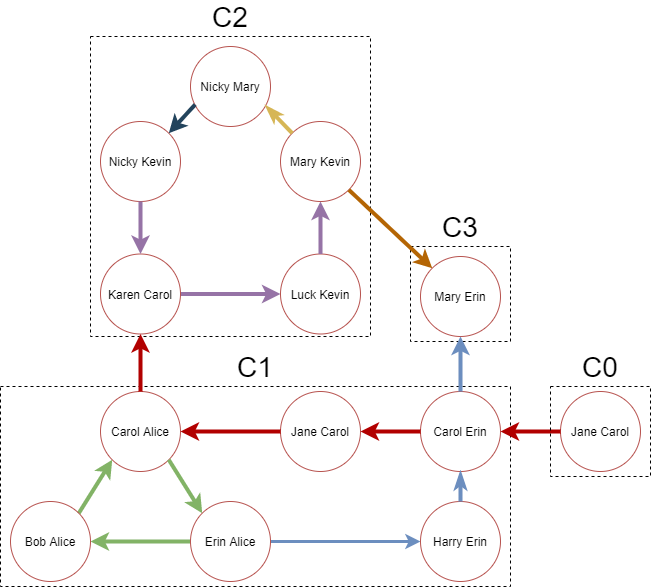
\includegraphics[width=\textwidth]{figures/uni-example.png}
    \caption{a tangle of four strongly connected components}
    \label{fig:uni-tangel}
\end{figure}

First, we prove that if every $c_i$ is concurrent, then there is a secure protocol. Since there is no cycle between $c_i$'s, there is a topological order between them. Consider the following algorithm.


\begin{algorithm}[H]
\label{alg:general_protocol}
\caption{Asynchronous Protocol}
\begin{algorithmic}
\State Let $\{c'_0, c'_1, .., c'_n\}$ is the topological order of $\mathcal{G}_s$ components.
\For{$i$ \textbf{from} $0$ \textbf{to} $n$}
\State Execute the synchronous protocol on $c'_i$
\EndFor
\end{algorithmic}
\end{algorithm}

Since each $c'_i$ is an cooperable tangle $T$, executing the synchronous protocol on each $c'_i$ is secure due to the result of theorem \ref{th:concurrency}. Hence, the entire execution process is secure.
% \begin{theorem}
% \label{th:opp-gen}
% Given a tangle $T$ and all of its strongly connected components in \genGraph graph $\{c_1, c_2, ..., c_n\}$, if there exists a $c_i$ which is not an executable concurrent tangle, then there is no tangle safe protocol for $T$.
% \end{theorem}
To prove the second direction of the theorem, we start by proving the following lemma:
\begin{lemma}
\label{lm:multiple-key-holder}
If there is a secure protocol for tangle $T$, then for each key, there is exactly one party who can own it.
\end{lemma}


We prove the lemma by contradiction. Assume in a concurrent tangle $T$ there are two parties $p_i$ and $p_j$ who are the key holder of the same lock. Then we prove that there is at least one party who may enter into the \underwater state. Given $\mathcal{G}_s=(V_g, E_g)$ assume $V_i \subset V$ and $V_j \subset V$ that for each $v \in V_i$, $p_i$ is the key holder and for each $v \in V_j$, $p_j$ is the key holder of the same stage. $\mathcal{G}_s$ is a strongly connected graph and for each $e \in E$ the same principal is overlapped between vertices $h(e)$ and $\tau(e)$, so the same lock is allowable on principals on both sides of $e$, hence $V_i \cap V_j$ can not be $\O$. Therefore, there is a swaption $s \in V_i \cap V_j$ that principals in $\beta(s)$ side and $\sigma(s)$ side are locked by different keys. Hence, if the key of one of these principals is revealed, its depositor will go \underwater.

% Therefore both parties in this swaption are threatened to be robbed and enter into underwater state. Because one of the $p_i$ may avoid to reveal its key while the other one reveals her key, then the principal which locked by the the revealed key will be transferred while other one will not. Thus the owner party of the transferred principal enters into the underwater state.

% that through the entire tangle there is no vertex $v$ that different locks are used for principal on vertices $v$ and $\mathcal{O}(v)$ in the same stage.
% swaption in which different locks are used for its outgoing black arcs. 
% Since 
% the outgoing arcs originating from the nodes of $p_1$ and $p_2$ have two different locks, whether there is two separately components on the \genGraph graph of the tangle or the same lock is used for all of the arcs in the tangle which is a contradiction. Thus there is a swaption which its ou\mathcal{G}_{t}oing black arcs are locked by different keys. Therefore The both parties in this swaption are threatened to be robbed and enter into underwater state. Because one of the $p_i$ may avoid to reveal its key while the other one reveals her key, then the arc which has the the revealed key will be triggered while other one will not. Thus the party corresponding to the triggered arc enters into underwater state.

% \ahC{Prove that source e $\mathcal{G}_{t}$ bayad keyone dastesh bashe.}

Now assume that there is a $c_i$ that is not cooperable tangle which means at least one of the following statements is true.

\begin{enumerate}
    \item $c_i$ is not \keyoneOk. Now, assume subgraph $\mathcal{G}_{t}=(V_t, E_t)$ of $\mathcal{G}_{p}$ for $c_i$ where $V_t=V$ and $E_t=\{e \in E | \rho(e) \neq t\}$. Then either $\mathcal{G}_{t}$ sources belong to different parties or the $\mathcal{G}_{p}$ has not any feedback edge set that satisfies the requirements of definition~\ref{def:pfok}. For the first case, there are at least two \keyone key holder parties in the graph. By the result of the lemma~\ref{lm:multiple-key-holder} there might be parties who go \underwater. In the second case, for each cycle $\mathcal{C}$ in $\mathcal{G}_{t}$ either for all edges $e \in \mathcal{C}$, $\rho(e)$ is $x$, thus the money transferring in $\mathcal{C}$ has to be the source of itself which is not acceptable, or for all edges $e \in \mathcal{C}$ that $\rho(e) \neq x$, $\tau(e)$ is not $p_{leader}$. If there is a protocol which executes $c_i$, to bypass this cycle, it must deviate from the principal deposition order imposed by edge $e \in \mathcal{C}$ that $\rho(e) \in \{i, t\}$. Hence the principal of the vertex $\tau(e)$ is forced to be deposited before the principal deposition of $h(e)$ while $\ell(\tau(e))$ is not $p_{leader}$. Then the party $\ell(h(e))$ can rob $\ell(\tau(e))$'s principal by cooperating with the graph key holders by early exposing all the keys.
    % there is at least one cycle $\mathcal{C}$ that 
    % has at least one insecure cycle. If there is more than one source in \keyoneGraph graph, then there are at least two parties in the graph who are the \keyone key holders. By the result of the lemma~\ref{lm:multiple-key-holder} it is a contradiction and there is a party who exits from the safe state. If there is an insecure cycle in the \keyoneGraphExtended graph, then there is a \textbf{Reversible} arc in this cycle. Since, if there is no such an arc in this cycle, then all of the arcs are black, hence the money which is transferring by these arcs has no source and comes from nowhere which is not acceptable. Therefore there must be at least one \textbf{Reversible} arc in this cycle. If there is a protocol which executes this tangle, to bypass the cycle, it must deviate from the principal deposition order imposed by one of the \textbf{Reversible} arcs in this cycle. Hence the party corresponding to the destination node of this arc is forced to deposit his principal before other party's deposition while he is none of the tangle key holders. Then the other party can robe his money by cooperating with the graph key holders by early exposing all the keys.
    
    % \ahC{We leave the case in which Bob deposits money from his own in multiple nodes} 
    
    % \ahC{alice and bob act as multiple nodes, it obviously fits in the scop of our proof}
    
    \item There is no party eligible to be the $p_{master}$ of $c_i$. 
   % \fatemeC{actually think pmaster is not defined on ci but anyway}:
    Then, if there is any protocol executing on $T$, then at least two locks are used for option funding stage. Hence, there is at least two key holders for the \Atwo key lock. Thus, there might be a party who goes \underwater.
    
\end{enumerate}

% Now we can define the swaptions universal theorem as a result of previously proved propositions:
% \begin{theorem}
% \label{th:universal}
% Given a tangle $T$, there is a safe protocol for executing $T$ if and only if every of $T$'s strongly connected components is an executable concurrent tangle.
% \end{theorem}


%\section{Conclusion}
\section{Conslusion}

In this paper, we first introduced ABD which is a single-chain bond contract. \new{Afterward,} by extending its design, we derived ABCD to achieve the goal of providing an interoperable cross-chain bond. Collectively, we have employed the well-known atomic cross-chain swaps for building ABCD as a primitive for uncollateralized DeFi. Potential use cases include but are not limited to exploiting arbitrage opportunities between swaptions without owning any capital or any other similar use case of flash loans and flash swaps with two major improvements: 
\begin{itemize}
    \item Despite the similarities, instead of being a ``flash'' loan which must be repaid within a block, \abcd can span an arbitrary long period of time for the issuer to trade or invest with the capital before the bond reaches maturity. The significance of this feature is highlighted by noting that this is not possible even in conventional financial systems to have an unsecured debt without a credit system. More precisely, this property is only possible due to full transparency and traceability of cryptocurrencies.
    \item Our proposed bond primitive does not require a Turing-complete programming language and bitcoin scripting language is sufficient to implement our method which is completely based on HTLC. While most DeFi protocols rely heavily on smart contracts or third parties which make them susceptible to security issues, \abcd can be flexibly used on the wide variety of HTLC-compatible blockchains and in particular, supports bitcoin natively.
\end{itemize}
 
%\section{Declaration of Interests}
\section{Declaration of Interests}
The authors declare that they have no known competing financial interests or personal relationships that could have appeared to influence the work reported in this paper.
%\section{The Elsevier article class}

%\paragraph{Installation} If the document class \emph{elsarticle} is not available on your computer, you can download and install the system package \emph{texlive-publishers} (Linux) or install the \LaTeX\ package \emph{elsarticle} using the package manager of your \TeX\ installation, which is typically \TeX\ Live or Mik\TeX.

%\paragraph{Usage} Once the package is properly installed, you can use the document class \emph{elsarticle} to create a manuscript. Please make sure that your manuscript follows the guidelines in the Guide for Authors of the relevant journal. It is not necessary to typeset your manuscript in exactly the same way as an article, unless you are submitting to a camera-ready copy (CRC) journal.

%\paragraph{Functionality} The Elsevier article class is based on the standard article class and supports almost all of the functionality of that class. In addition, it features commands and options to format the
%\begin{itemize}
%\item document style
%\item baselineskip
%\item front matter
%\item keywords and MSC codes
%\item theorems, definitions and proofs
%\item lables of enumerations
%\item citation style and labeling.
%\end{itemize}

%\section{Front matter}

%The author names and affiliations could be formatted in two ways:
%\begin{enumerate}[(1)]
%\item Group the authors per affiliation.
%\item Use footnotes to indicate the affiliations.
%\end{enumerate}
%See the front matter of this document for examples. You are recommended to conform your choice to the journal you are submitting to.

%\section{Bibliography styles}

%There are various bibliography styles available. You can select the style of your choice in the preamble of this document. These styles are Elsevier styles based on standard styles like Harvard and Vancouver. Please use Bib\TeX\ to generate your bibliography and include DOIs whenever available.

%Here are two sample references: %\cite{Feynman1963118,Dirac1953888}.

%\section{References}

\bibliography{sections/bibliography.bib}

\end{document}